\documentclass[9pt]{beamer}
%\usepackage[margin=0.1in]{geometry}
\usepackage{skull} % for skull symbol
\usepackage{graphicx}
\usepackage{amsmath, amssymb}
\usepackage{multirow}
\usepackage{cite}
%\usepackage{mathabx} % for convolution symbol
\usepackage{pgfplots} % for tikzpicture
\usepackage{color}
\usepackage{tikz}
%\usepackage{pgf}
%\usetikzlibrary{shapes,matrix}
\usetikzlibrary{matrix}

\def\layersep{1.5cm}

% for colored math symbols
\newcommand*{\mathcolor}{}
\def\mathcolor#1#{\mathcoloraux{#1}}
\newcommand*{\mathcoloraux}[3]{%
  \protect\leavevmode
  \begingroup
    \color#1{#2}#3%
  \endgroup
}

\mode<notes>{
%\usetheme{Berkeley}
\definecolor{uofsgreen}{rgb}{0.125,0.5,0.25}
\usecolortheme[named=uofsgreen]{structure}
}

\setbeamerfont{page number in head/foot}{size=\large}
\setbeamertemplate{footline}[frame number]

%\title[Short Paper Title]{Dermatologist-level classification of skin cancer with deep neural networks}
%\subtitle{A. Esteva, B. Kuprel, R.A. Novoa, J. Ko, S.M. Swetter, 
%H.M. Blau, and S. Thrun} % (optional)
\title[Short Paper Title]{CNN Architectures for Image Classification}
\subtitle{}
%\author{Shubhra Aich}
\institute{}
\author{\texorpdfstring{Shubhra Aich\newline\url{s.aich.72@gmail.com}}{Shubhra Aich}}
\date{January 17, 2018}


\begin{document}


\nocite{*}

\begin{frame}
  \titlepage
\end{frame}

\begin{frame}
  \frametitle{Architectures}
  \tableofcontents
\end{frame}

%\section{Architectural Overview}

\subsection{LeNet5}
\begin{frame}
	\frametitle{LeNet5(1998)}
	\begin{minipage}[t]{0.45\textwidth}	
		\begin{figure}[t]
			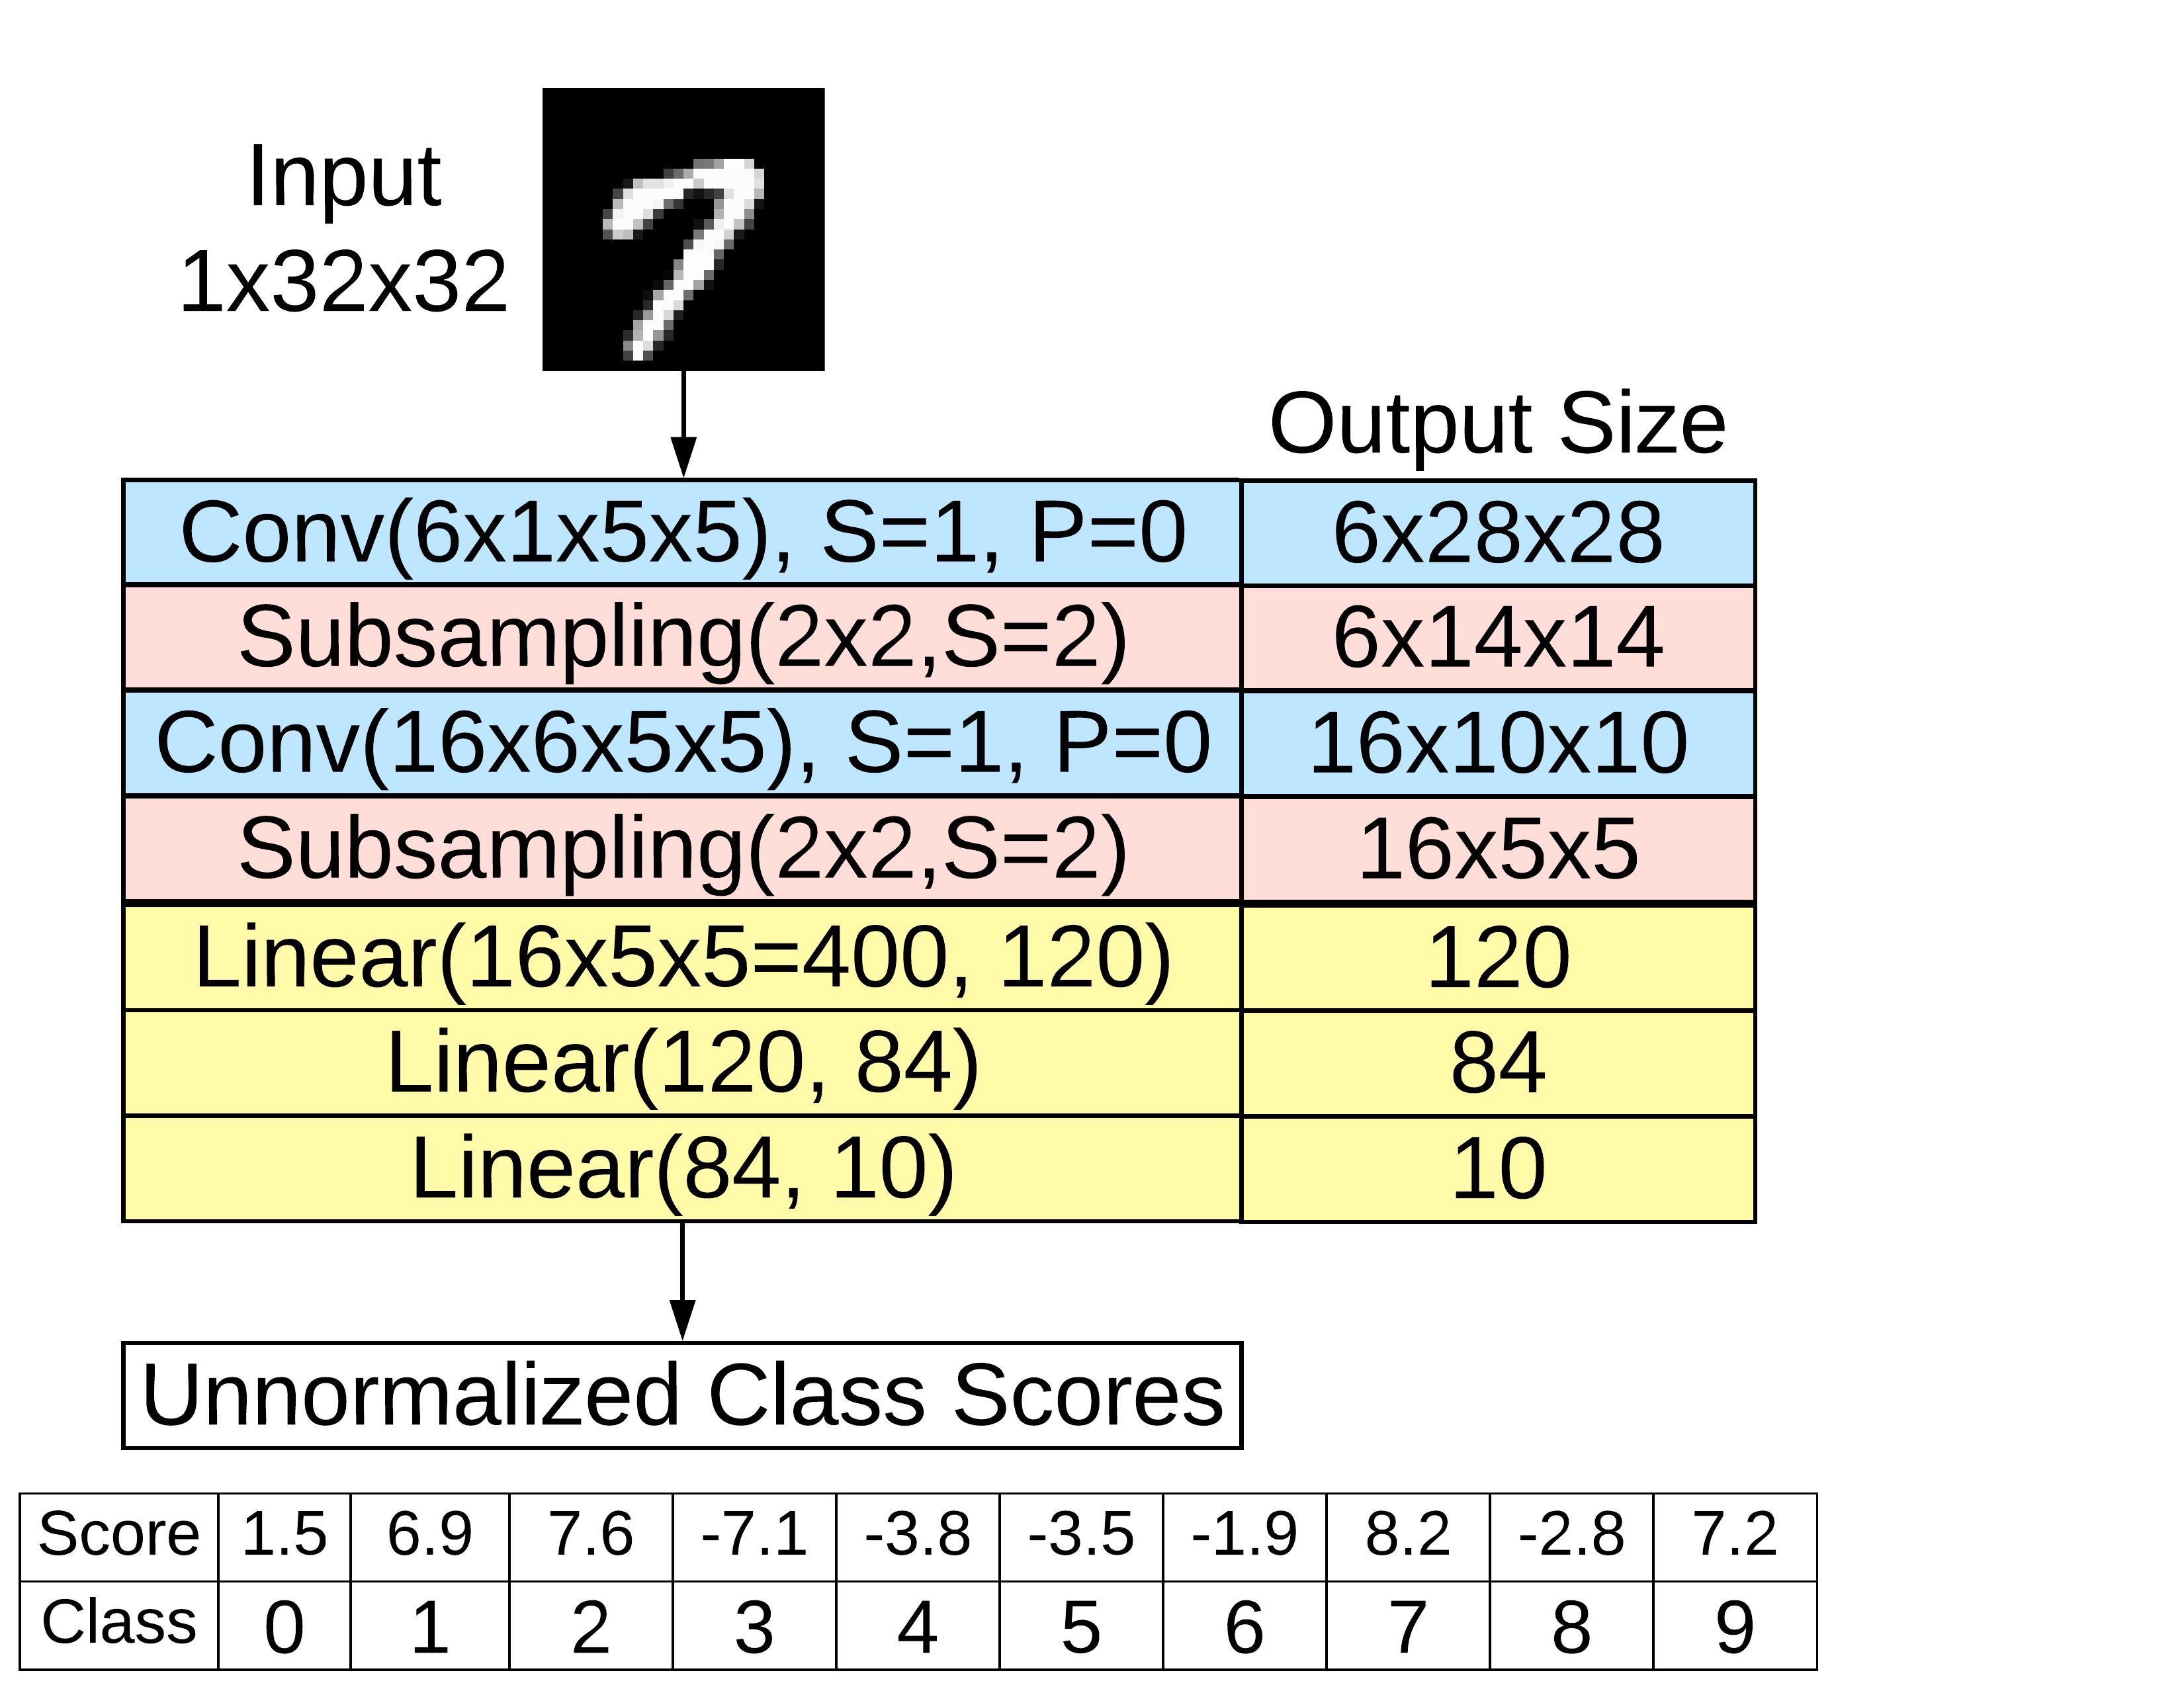
\includegraphics[scale=0.06]{./figures/edit/lenet5.png}
		\end{figure}
	\end{minipage}	\hspace{1.0cm}
	\begin{minipage}[t]{0.40\textwidth}
		\begin{figure}
	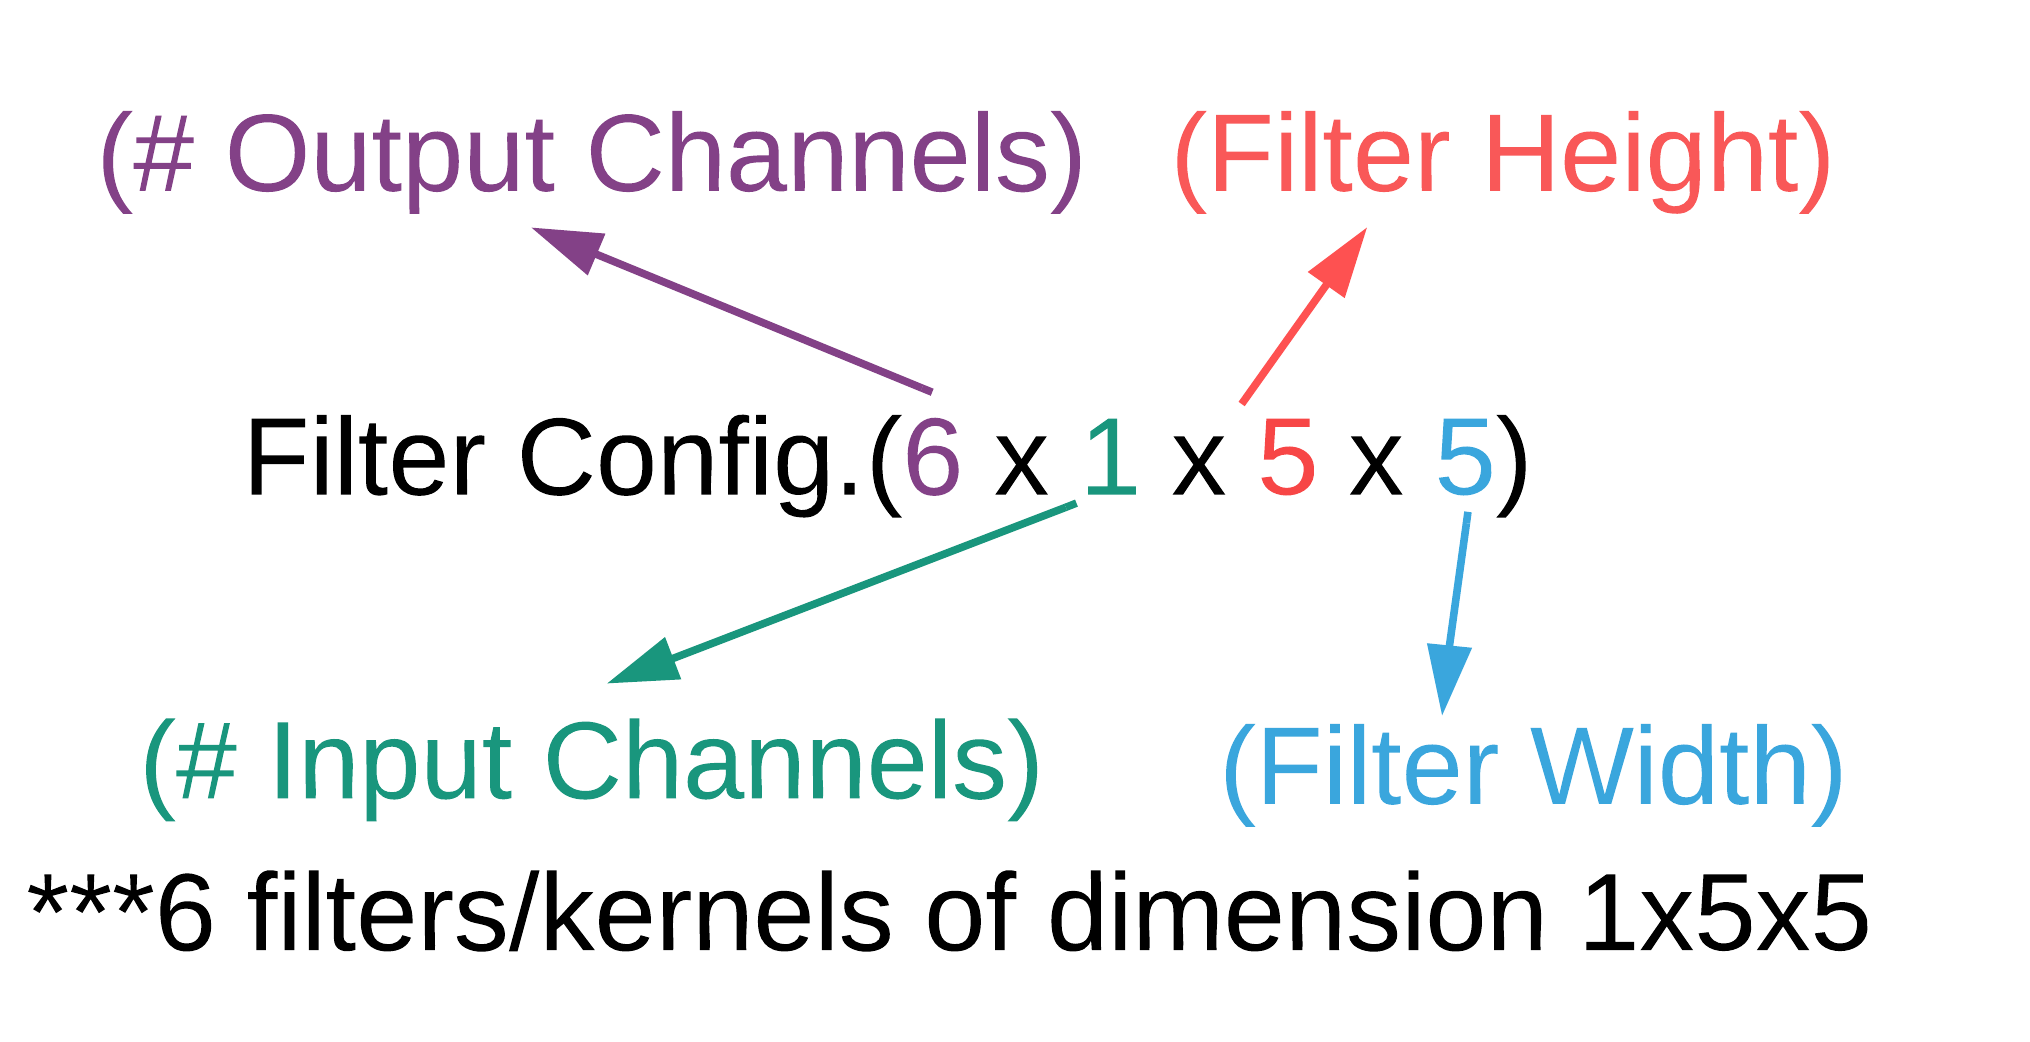
\includegraphics[scale=0.07]{./figures/edit/filter_config.png} 				
	\end{figure} \\
	
	$M_{new} = \frac{M_{old} + 2P - F}{S} + 1$ \\
	\small $M_{old} = 32$, \\ 
	\small $Stride(S) = 1$, \\ 
	\small $Padding(P) = 0$ \\
	\small $M_{new} = \frac{32 + 2\times0 - 5}{1} + 1 = 28$ 
	\end{minipage} 
\end{frame}

\subsection{AlexNet}
\begin{frame}
	\frametitle{AlexNet(2012)}
	\begin{minipage}[t]{\textwidth}	
		\begin{figure}[t]
			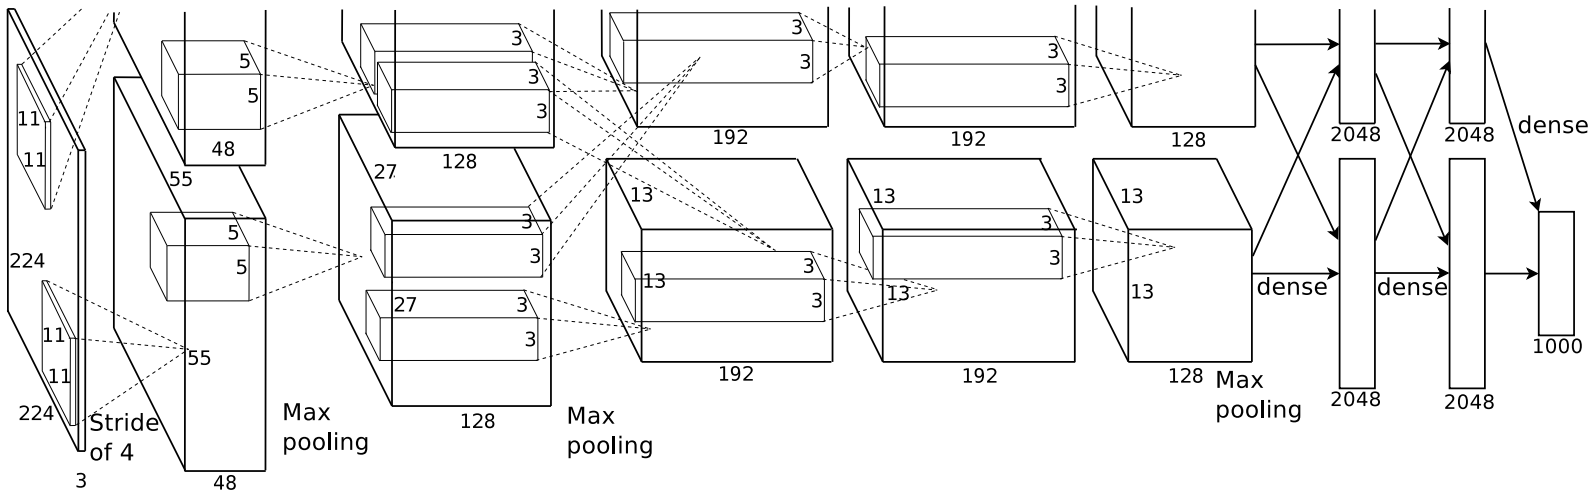
\includegraphics[scale=0.18]{./figures/edit/alexnet_original.png}
		\end{figure}
	\end{minipage}	\\
	\begin{minipage}[t]{0.35\textwidth}	
		\begin{figure}[t]
			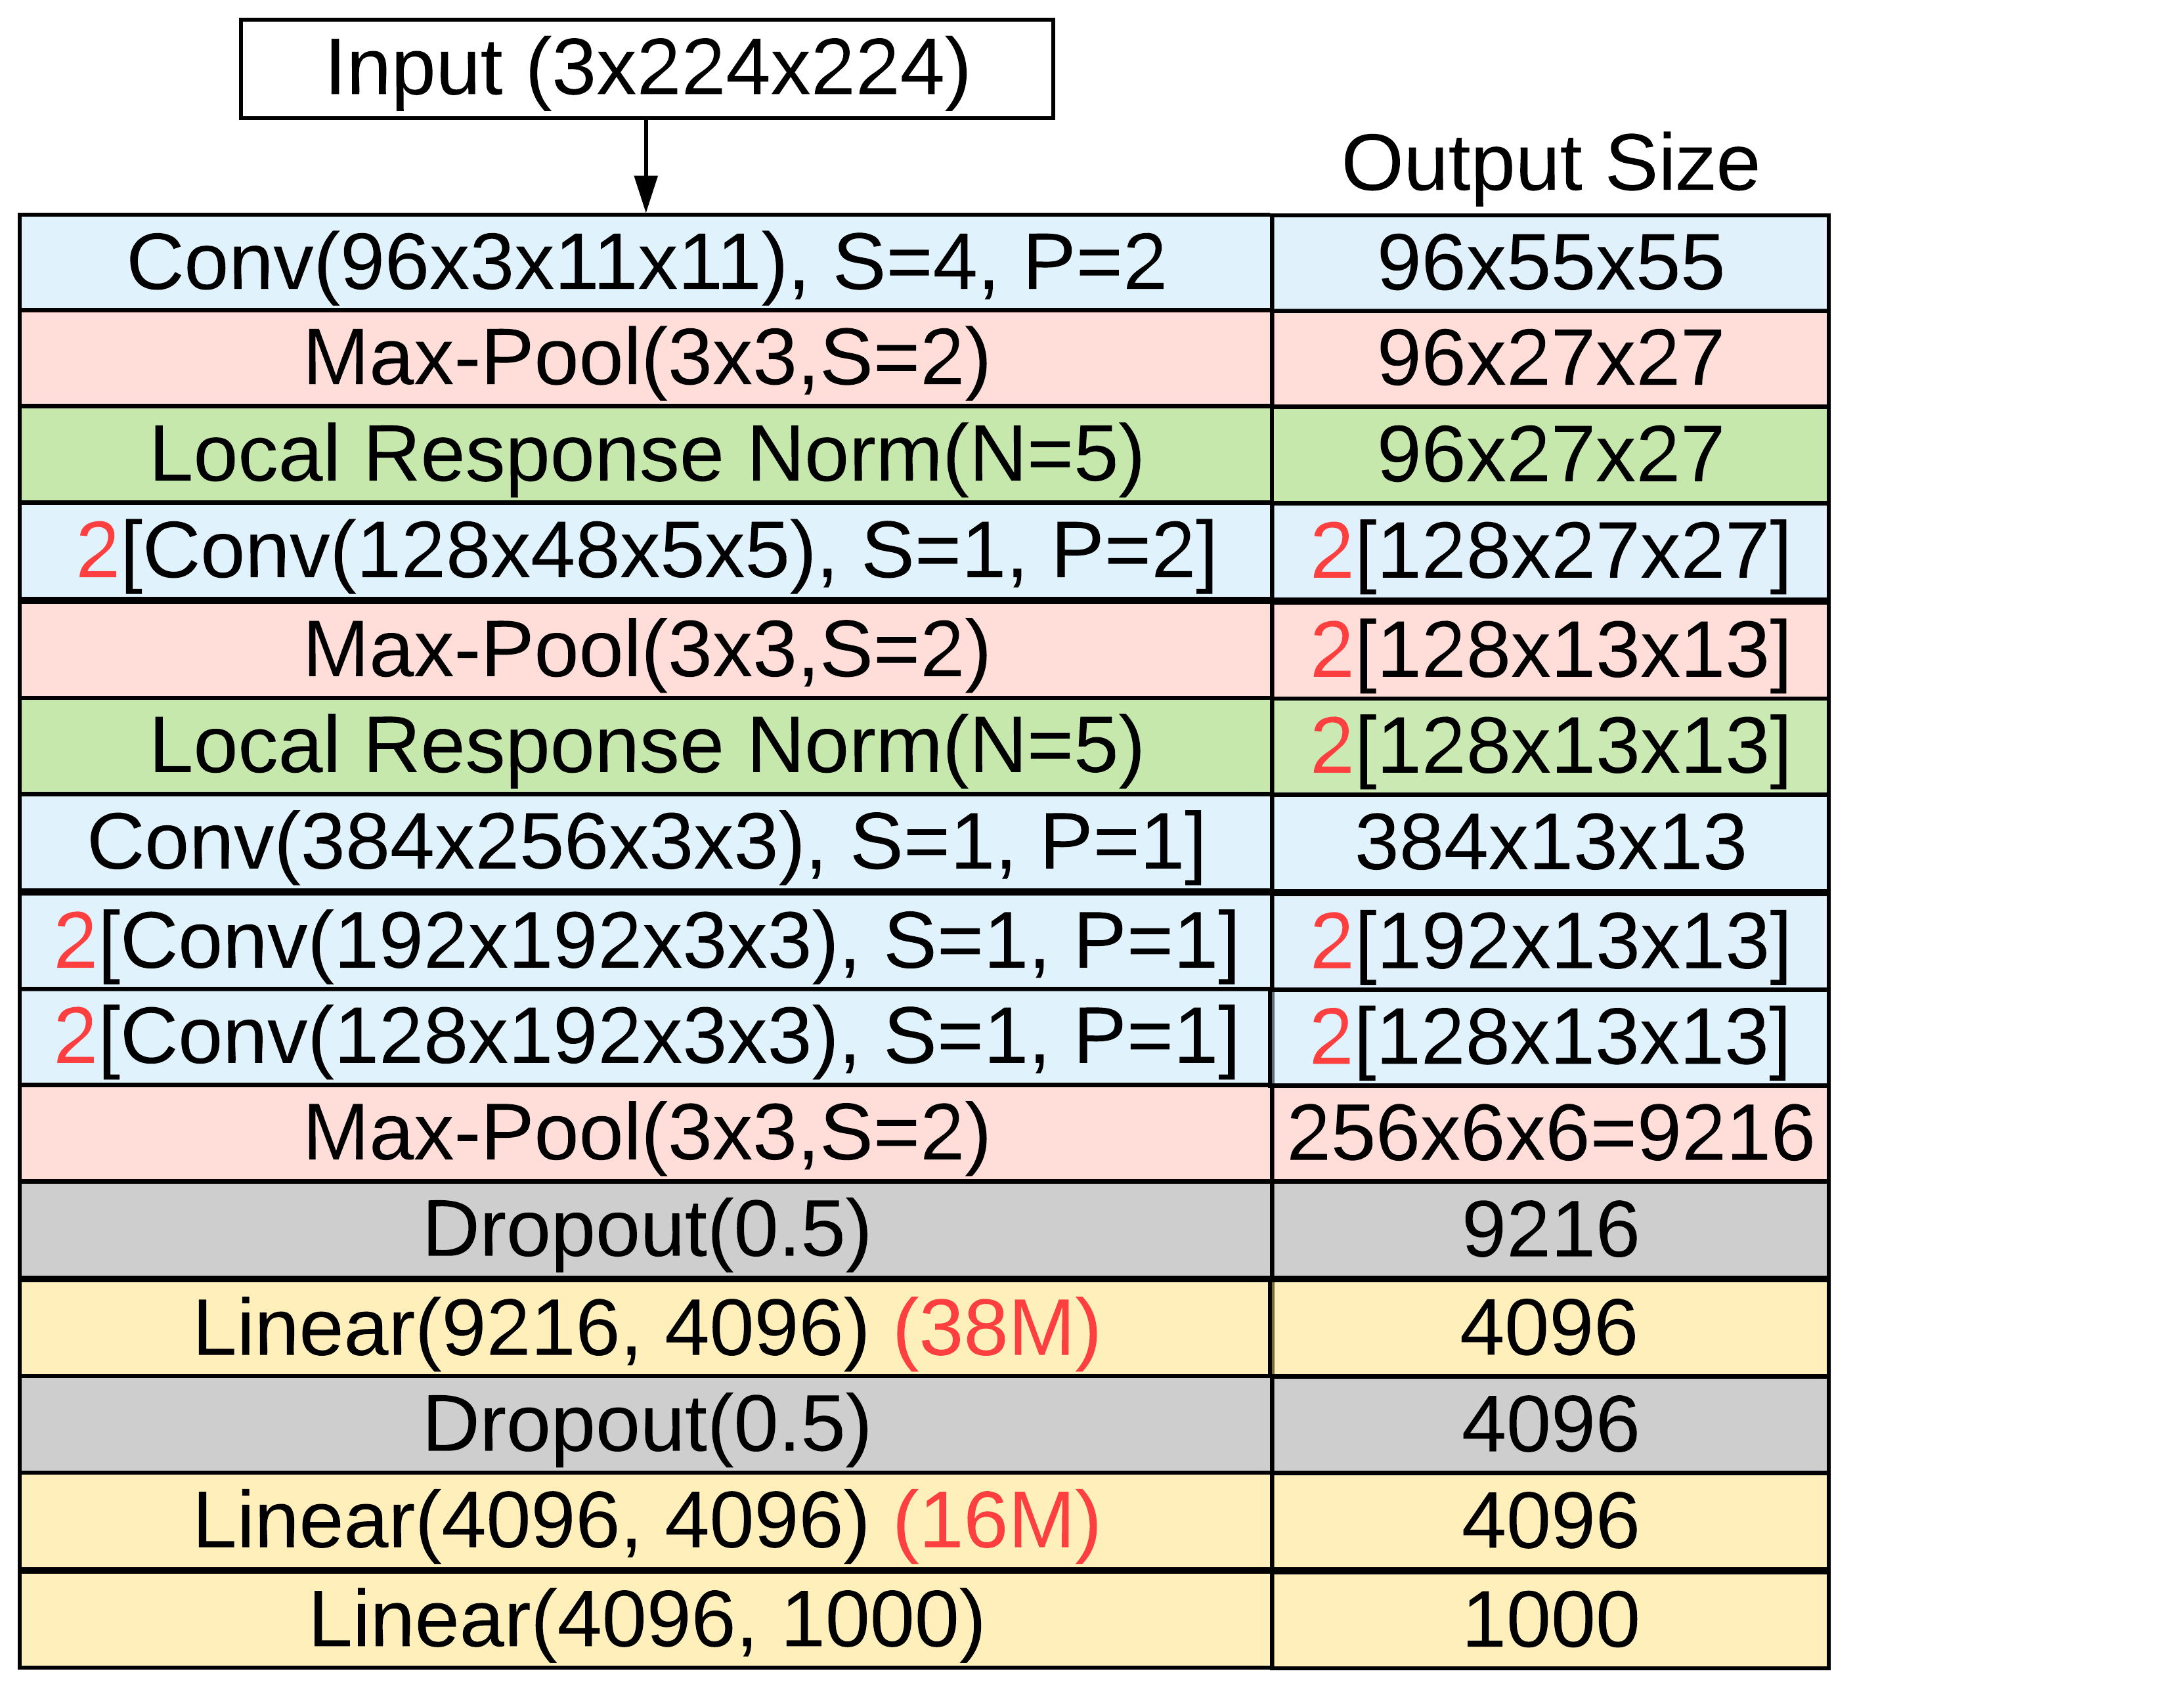
\includegraphics[scale=0.045]{./figures/edit/alexnet.png}
		\end{figure}
	\end{minipage}	\hspace{1.5em}
	\pause
	\hspace{1.0em}\begin{minipage}[t]{0.55\textwidth}	
		\vspace{1.5em}
		Novelties/Significance
		\begin{itemize}
			\item \small GPU implementation (2xNVIDIA GTX 580 3GB GPUs).
			\item \small ReLU as nonlinearity.
			\item \small Local Response Normalization (LRN).
			\item \small Data augmentation.
			\item \small $\sim10\%$ improvement on standard benchmark compared to traditional approaches.
		\end{itemize}
	\end{minipage}		
\end{frame}

\begin{frame}
	\frametitle{Data Augmentation}
	\begin{minipage}[t]{\textwidth}	
		\begin{itemize}
			\item \small Trained on ImageNet dataset comprising $\sim1.2M$ training samples.
			\item \small $5$ $(224\times 224)$ patch extraction from each training samples.
					\begin{itemize}
						\item[--] 4 from 4 corners + 1 from the center.
						\item[--] horizontal flipping of 5 patches gives 10 patches/image.
						\item[--] averaging the scores from $10$ $(224\times 224)$ patches in test phase.
					\end{itemize}
			\item \small Obtained illumination invariance of the object identities using the PCA trick : \\ ~ \\
			\begin{multiline} 
    				\begin{bmatrix}
        				r(x,y) \\ g(x,y) \\ b(x,y)
    				\end{bmatrix}
    				+= 
    				\begin{bmatrix}
        				| & | & | \\
        				e_1 & e_2 & e_3 \\
        				| & | & |
    				\end{bmatrix}
    				\begin{bmatrix}
        				\alpha_1 \lambda_1 \\ \alpha_2 \lambda_2 \\ \alpha_3 \lambda_3 
    				\end{bmatrix}	\\~\\
    				\alpha_i \sim \mathcal{N}(0,0.1)							
			\end{multiline}

		\end{itemize}
	\end{minipage}		
\end{frame}

\begin{frame}
	\frametitle{Local Response Normalization}
	\begin{minipage}[t]{\textwidth}	
		\begin{equation}
			b_{x,y}^{k} = 
			\frac{a_{x,y}^{k}}
			{\left(\gamma + \alpha \sum_{i=max(0,N/2)}^{min(D-1, k-N/2)} {\left(a_{x,y}^{i}\right)^2}\right)^\beta}
		\end{equation}
		\begin{multiline}
			a_{x,y}^{k} = \text{unnormlized activity generated by the kernel $k$ at position $(x,y)$} \\
			b_{x,y}^{k} = \text{normalized activity corresponding to} \hspace{0.2em}a_{x,y}^{k} \\
			D = \text{total number of kernels/feature maps} \\
			\alpha, \beta, \gamma, N \text{-- determined using the validation set.}
		\end{multiline}		
		\vspace{1em}
		\begin{itemize}
			\item Imposes lateral inhibition amongst the neighboring elements in the feature maps.			
		\end{itemize}
	\end{minipage}		
\end{frame}

\begin{frame}
	\frametitle{Results-AlexNet}
		\begin{itemize}
			\item Trained for 90 epochs on $1.2M$ images for $5-6$ days using 2xNVIDIA GTX 580 3GB GPUs 
		\end{itemize}	
		\begin{table}[]
		\centering
		\caption{ILSVRC 2010 Test Set}
		\label{my-label}
		\begin{tabular}{|c|c|c|}
		\hline
		\multirow{2}{*}{Method} & \multicolumn{2}{c|}{Error (\%)} \\ \cline{2-3} 
		 & Top-1 & Top-5 \\ \hline
		SIFT + FV & 45.7 & 25.7 \\ \hline
		AlexNet & 37.5 & 17.0 \\ \hline
		\end{tabular}
		\end{table}
\end{frame}

\subsection{VGG}
\begin{frame}
	\frametitle{VGG(2014)}
		\begin{itemize}
			\item Equivalence of spatial coverage :
				\begin{itemize}
					\item[o] 1 $(5\times 5)$ convolution $\equiv$ 2 $(3\times 3)$ convolutions
					\item[o] 1 $(7\times 7)$ convolution $\equiv$ 3 $(3\times 3)$ convolutions
				\end{itemize} 
			\item Using smaller convolution kernels is computationally efficient :
				\begin{itemize}
					\item[o] 1 $(5\times 5)$ convolution has 25 training parameters, whereas 2 $(3\times 3)$ convolutions comprise 18 training parameters.
					\item[o] 1 $(7\times 7)$ convolution has 49 training parameters, whereas 3 $(3\times 3)$ convolutions comprise 27 training parameters.
				\end{itemize} 				
			\item (Smaller kernels + More Depth) $\equiv$ More Nonlinearity $\equiv$ Better Modeling.					
		\end{itemize}
		\pause
		\begin{figure}
			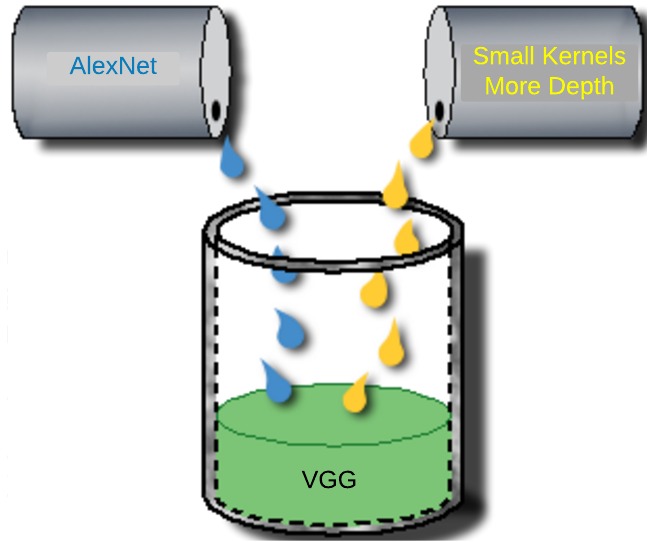
\includegraphics[scale=1.0]{./figures/edit/vgg_mixture.png}
		\end{figure}			
\end{frame}

\begin{frame}
	\frametitle{AlexNet vs. VGG16}
		\begin{figure}[t]
			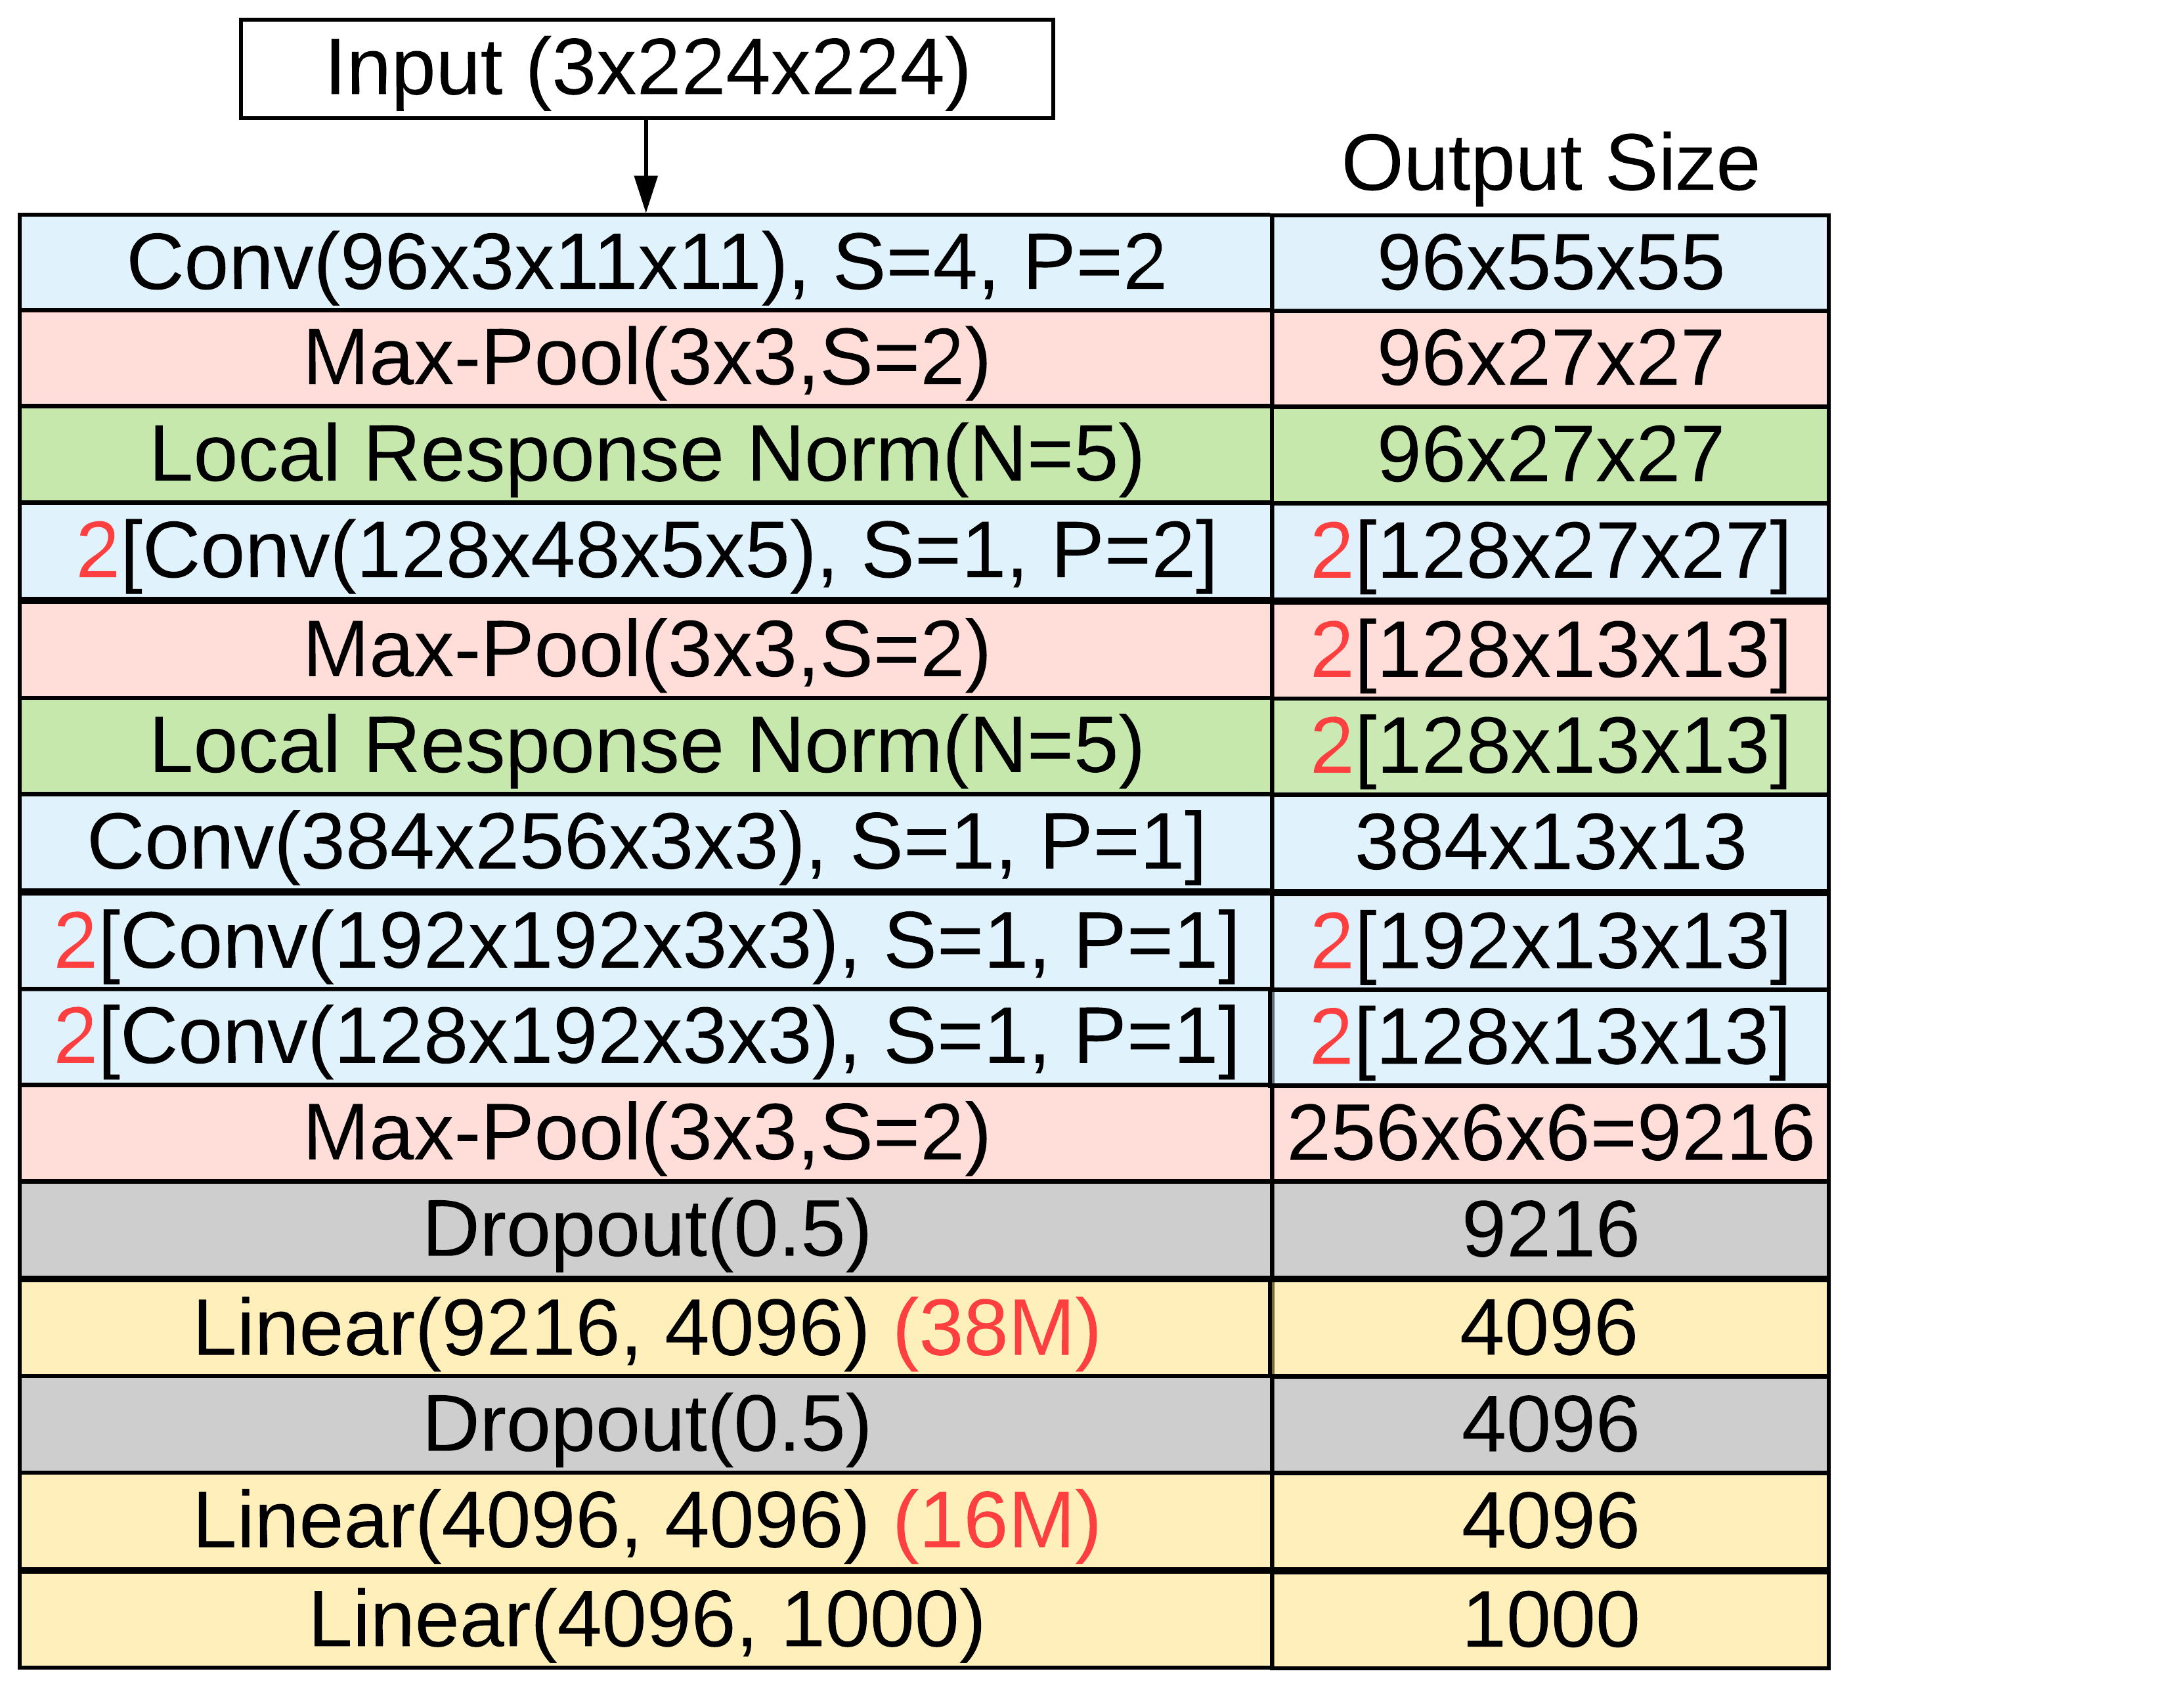
\includegraphics[scale=0.05]{./figures/edit/alexnet.png}
			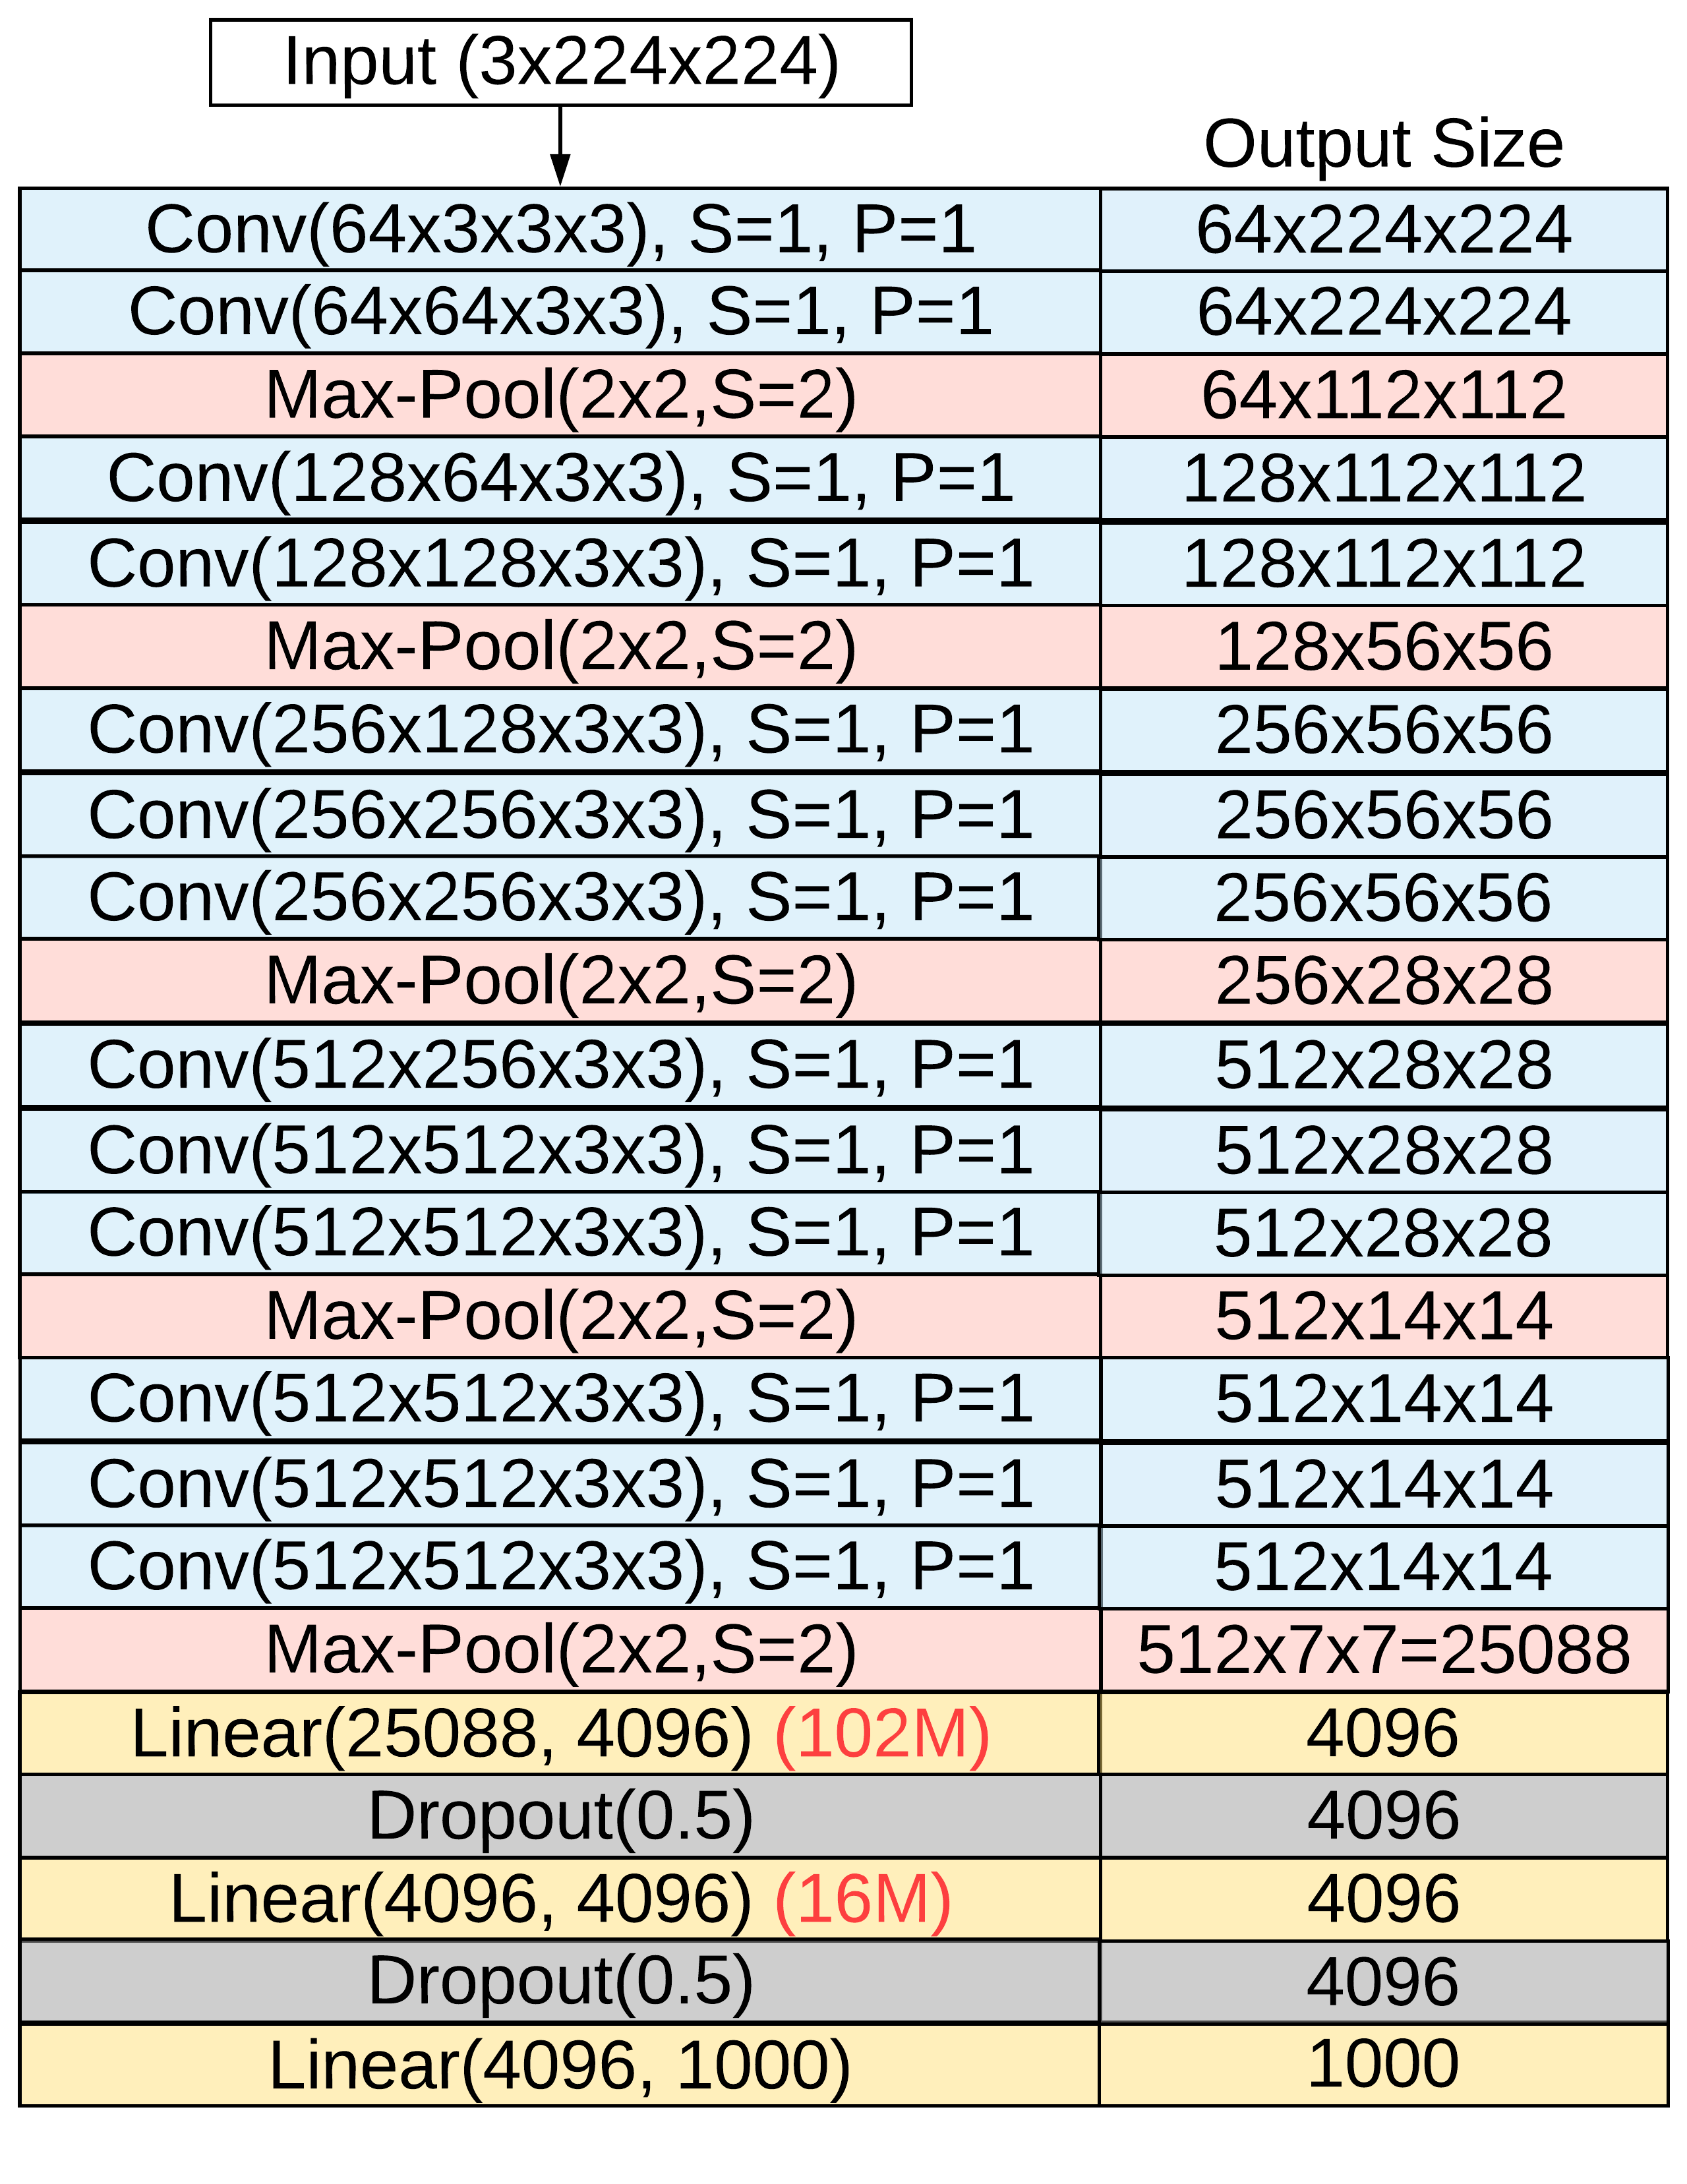
\includegraphics[scale=0.05]{./figures/edit/vgg.png}
		\end{figure}	
		\pause	
		\begin{itemize}
			\item AlexNet: variable size kernels based on heuristics, hard to modify.
			\item VGG: deeper network with fixed size kernels, so comparatively easier to play with, no use of LRN.
		\end{itemize} 			
\end{frame}

\begin{frame}
	\frametitle{Training VGG}
		\begin{itemize}
			\item VGG is deeper -- hard to train with Gaussian initialization.
			\item Pre-initialization with smaller nets (version A).
			\item Training with multi-scale inputs.
			\item Dense evaluations (150 per sample) at the test time.
			\begin{figure}
				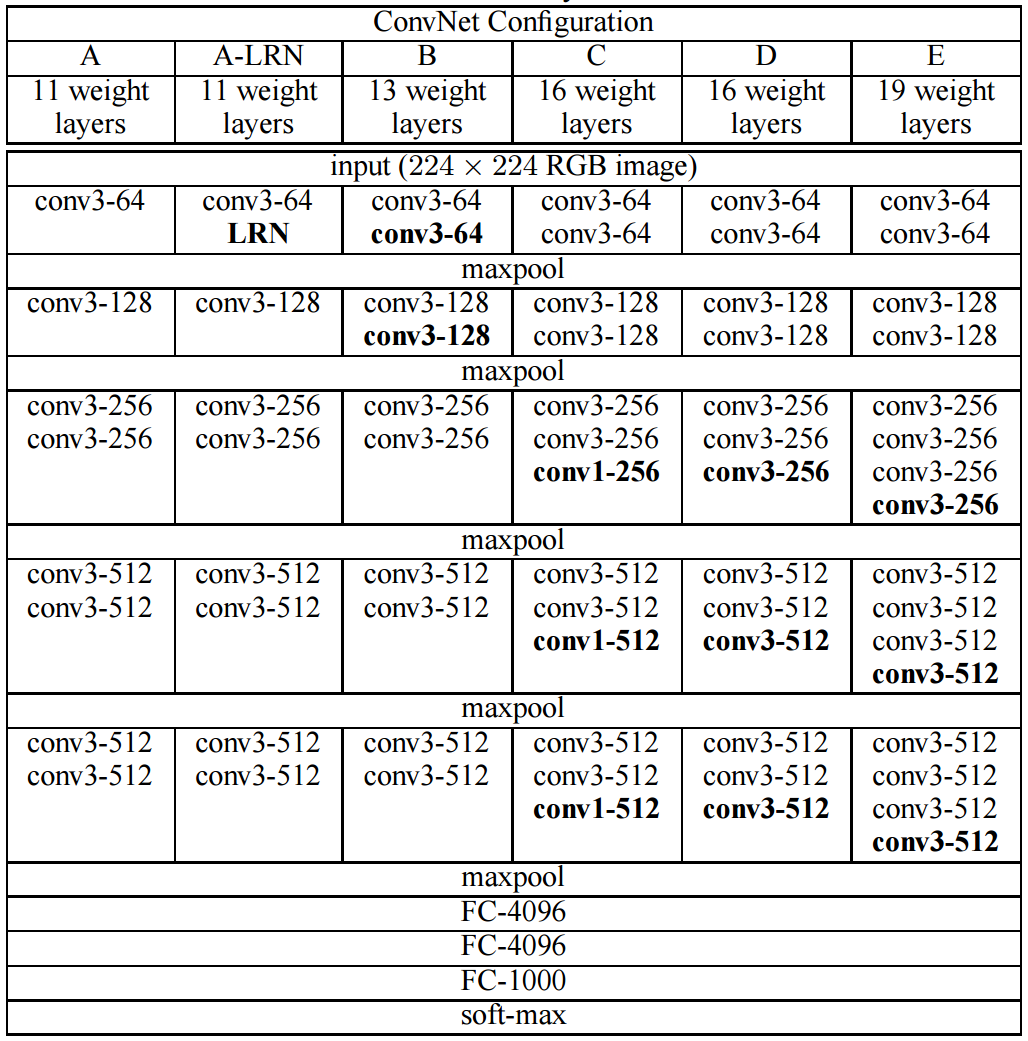
\includegraphics[scale=0.14]{./figures/edit/vgg_all.png}
			\end{figure}
		\end{itemize}
		\pause	
		
\includegraphics[scale=0.01]{./figures/edit/eureka-min.jpg}  \hspace{0.5em}Possible to train from scratch with Xavier-Glorot(2010) initialization !!!	
\end{frame}

\begin{frame}
	\frametitle{Results-VGG}
		\begin{itemize}
			\item Training on $1.2M$ ImageNet samples with 4xNVIDIA TITAN Black 6GB GPUs takes $2-3$ weeks depending on the architecture.
		\end{itemize}	
		\begin{table}[]
		\centering
		\label{my-label}
		\begin{tabular}{|c|c|c|}
		\hline
		\multirow{2}{*}{Method} & \multicolumn{2}{c|}{Error (\%)} \\ \cline{2-3} 
		 & Top-1 & Top-5 \\ \hline
		SIFT + FV & 45.7 & 25.7 \\ \hline
		AlexNet & 37.5 & 17.0 \\ \hline
		VGG16 & 24.4 & 7.2 \\ \hline
		VGG19 & 24.4 & 7.1 \\ \hline
		\end{tabular}
		\end{table}
\end{frame}

\subsection{Inception}
\begin{frame}
	\frametitle{We Need More Nonlinearity}
		\begin{itemize}
			\item Using small kernels $(3\times 3) \implies$ VGG.
			\item Theoretically, high-dimensional data space demands more non-linearity in the models.
				\begin{itemize}
					\item[--] Training deeper networks (did not work until 2015).
					\item[--] Replacement of linear convolution operation with a non-linear operation -- \textbf{Nested Network} or \textbf{Network in Network}.
				\end{itemize}				
		\end{itemize}
		\pause	
	\begin{figure}
		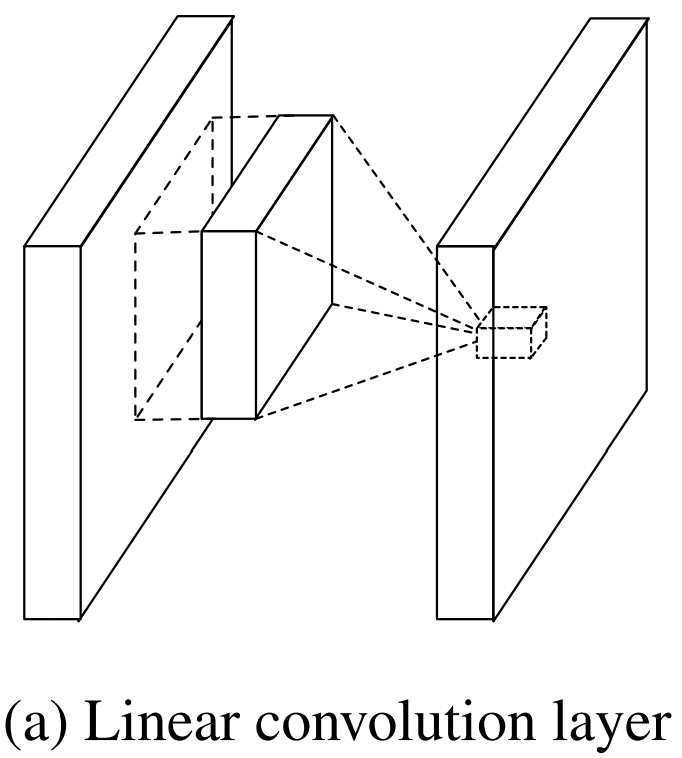
\includegraphics[scale=0.15]{./figures/edit/nin_01.png} \hspace{2em}
		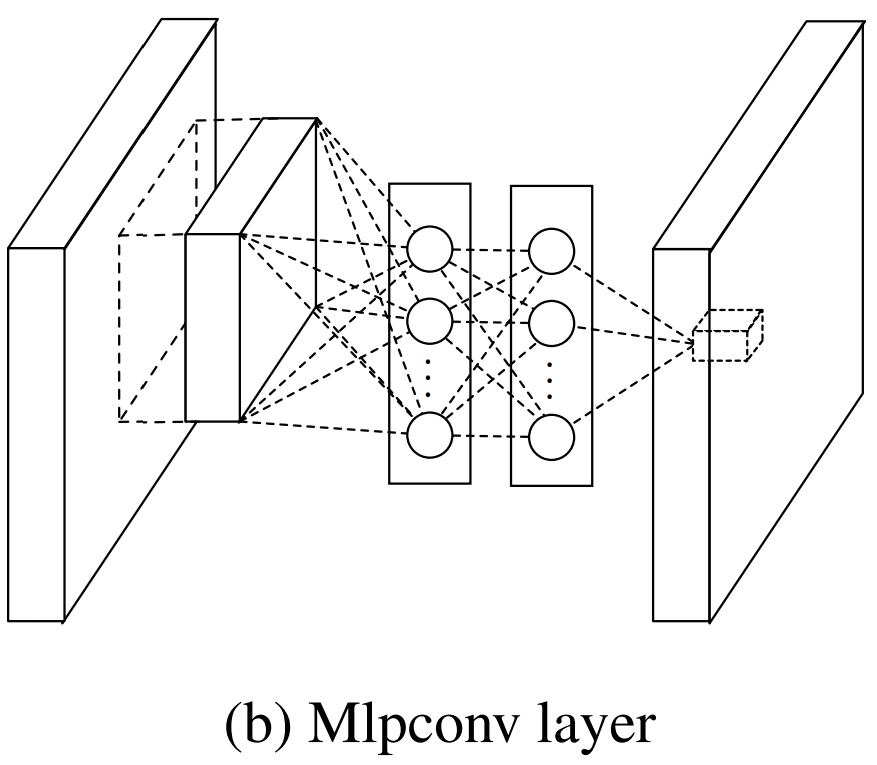
\includegraphics[scale=0.15]{./figures/edit/nin_02.png} \\			
	\end{figure}		
\end{frame}

\begin{frame}
	\frametitle{Network In Network (NIN)}
	\begin{figure}
		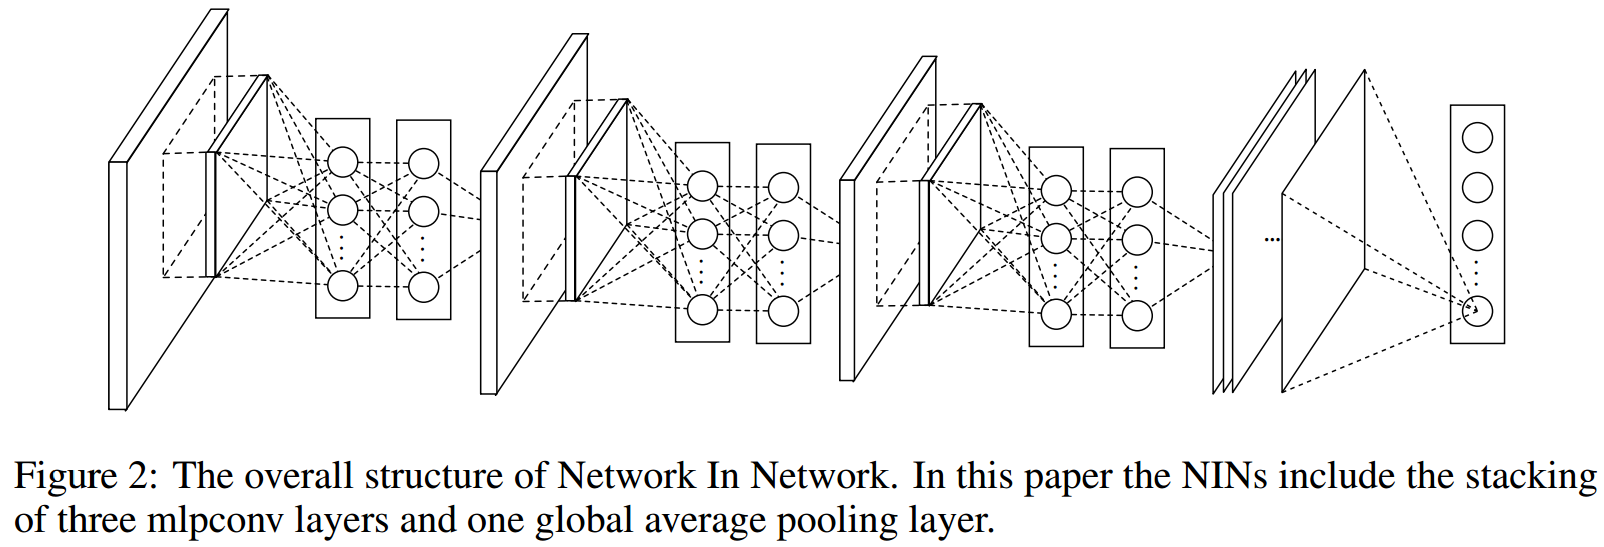
\includegraphics[scale=0.2]{./figures/edit/nin_03.png} 				
	\end{figure}
		\begin{itemize}
			\item Replacement of linear convolution with MLP-NN.
			\item Replacement of \textcolor{red}{HUGE (!!!) Fully-Connected (FC)} layers with a single \textcolor{green!70!black}{Global Average Pooling (GAP)} layer
				\begin{itemize}
					\item[--] More than $90-95\%$ reduction of training parameters $\implies$ much less prone to overfitting.
					\item[--] More emphasis on convolutional features (head of the architecture).
				\end{itemize} 
		\end{itemize}	
\end{frame}

\begin{frame}
	\frametitle{Paradigm Shift}
	\hspace{0.5em}\textcolor{red!70!black}{Heavy-Tail (AlexNet, VGG)} $\rightarrow$ \textcolor{green!70!black}{Heavy-Head (NIN, Inception, ...)}
	\pause
	\begin{figure}
		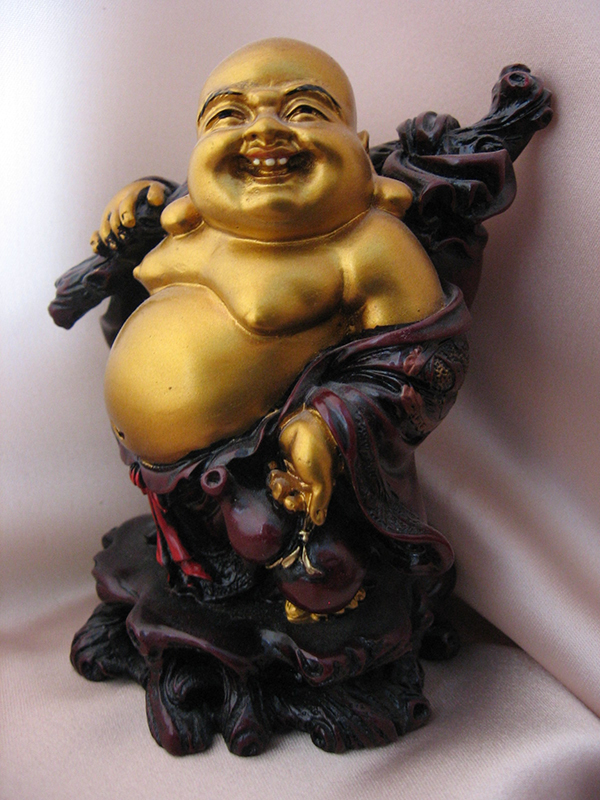
\includegraphics[scale=0.4]{./figures/edit/heavy-tail.jpg} \hspace{1.5em}
		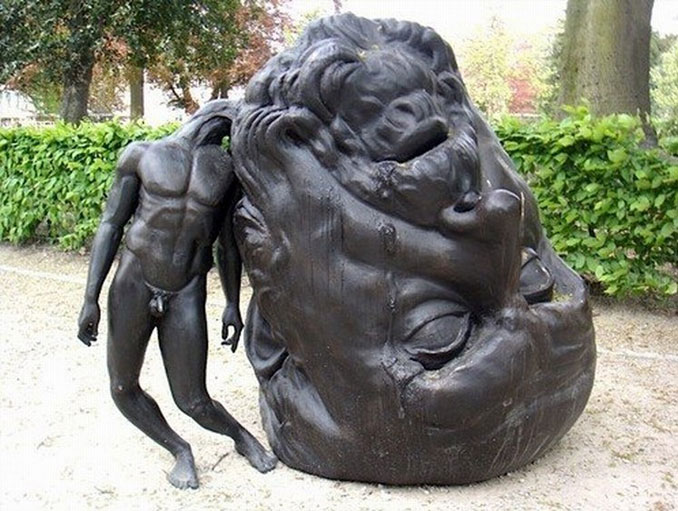
\includegraphics[scale=0.25]{./figures/edit/heavy-head.jpg} 	
	\end{figure}	
\end{frame}

\begin{frame}
	\frametitle{Breaking down Convolution ... (1)}
	\begin{itemize}
	\item Straightforward $5 \times 5$ convolution \\
	M $\equiv$ Multiplication and A $\equiv$ Addition \\
	\end{itemize}
	\begin{minipage}{.4\textwidth}
		\begin{tikzpicture}

    	%\matrix[matrix of nodes,nodes={draw},row 										1 2/.style={nodes={fill=blue!20}}] {
    	\matrix (m) [matrix of nodes,
    		nodes={rectangle,draw, fill=blue!10} ]{
      			$a_{11}$ && $a_{12}$ && $a_{13}$ && $a_{14}$ && $a_{15}$ \\ 
      			$a_{21}$ && $a_{22}$ && $a_{23}$ && $a_{24}$ && $a_{25}$ \\ 
      			$a_{31}$ && $a_{32}$ && $a_{33}$ && $a_{34}$ && $a_{35}$ \\ 
      			$a_{41}$ && $a_{42}$ && $a_{43}$ && $a_{44}$ && $a_{45}$ \\ 
      			$a_{51}$ && $a_{52}$ && $a_{53}$ && $a_{54}$ && $a_{55}$ \\       		};
  		\end{tikzpicture}
  	\end{minipage}
  	\begin{minipage}{0.05\textwidth}
  		\ast
  	\end{minipage}
	\begin{minipage}{0.36\textwidth}  	
		\begin{tikzpicture}

    	%\matrix[matrix of nodes,nodes={draw},row 										1 2/.style={nodes={fill=blue!20}}] {
    	\matrix (m) [matrix of nodes,
    		nodes={rectangle,draw, fill=blue!10} ]{
      			$h_{11}$ && $h_{12}$ && $h_{13}$ && $h_{14}$ && $h_{15}$ \\ 
      			$h_{21}$ && $h_{22}$ && $h_{23}$ && $h_{24}$ && $h_{25}$ \\ 
      			$h_{31}$ && $h_{32}$ && $h_{33}$ && $h_{34}$ && $h_{35}$ \\ 
      			$h_{41}$ && $h_{42}$ && $h_{43}$ && $h_{44}$ && $h_{45}$ \\ 
      			$h_{51}$ && $h_{52}$ && $h_{53}$ && $h_{54}$ && $h_{55}$ \\  		};
  		\end{tikzpicture}	
  	\end{minipage} \\
  	$ output_{33} = a_{11}h_{11} + a_{12}h_{12} + \dots  + a_{31}h_{31} + a_{32}h_{32} + \dots + a_{54}h_{54} + a_{55}h_{55} $ \\
  	$\mathcolor{red}{ \equiv } $ \textcolor{red}{25M + 24A} \\
  	The filter ($h_{ij}$) will slide over the image ($a_{ij}$) for each position once totalling $25$ times. \\
  	So, total number of gross multiplication and addition  \textcolor{red}{= 25(25M + 24A) = 625M + 600A}
  	  
\end{frame}

\begin{frame}
	\frametitle{Breaking down Convolution ... (2)}
	\begin{itemize}
	\item Breaking down $5 \times 5$ convolution into 2 consecutive 
		 $3 \times 3$ convolutions 
		 \begin{itemize}
		 	\item Step - 01: Convolving $5 \times 5$ matrix with $3 \times 3 filter$
		 \end{itemize}
	\end{itemize}
	\begin{minipage}{.38\textwidth}
    \begin{tikzpicture}
    \matrix (m) [matrix of nodes,
        nodes={rectangle,draw, fill=blue!10} ]{
            $a_{11}$ && $a_{12}$ && $a_{13}$ && $a_{14}$ && $a_{15}$ \\
            $a_{21}$ && $a_{22}$ && $a_{23}$ && $a_{24}$ && $a_{25}$ \\
            $a_{31}$ && $a_{32}$ && $a_{33}$ && $a_{34}$ && $a_{35}$ \\
            $a_{41}$ && $a_{42}$ && $a_{43}$ && $a_{44}$ && $a_{45}$ \\
            $a_{51}$ && $a_{52}$ && $a_{53}$ && $a_{54}$ && $a_{55}$ \\       		};
    \draw [thick, red] (m-1-1.north west) -- (m-1-3.north east) -- (m-3-3.south east) -- (m-3-1.south west) -- cycle ;
    \draw [thick, blue] (m-1-3.north west) -- (m-1-5.north east) -- (m-3-5.south east) -- (m-3-3.south west) -- cycle ;
    \draw [thick, cyan] (m-3-1.north west) -- (m-3-3.north east) -- (m-5-3.south east) -- (m-5-1.south west) -- cycle ;
    \end{tikzpicture}
\end{minipage}
\begin{minipage}{0.01\textwidth}
    \ast
\end{minipage}
\begin{minipage}{0.23\textwidth}
    \begin{tikzpicture}

    %\matrix[matrix of nodes,nodes={draw},row 										1 2/.style={nodes={fill=blue!20}}] {
    \matrix (m) [matrix of nodes,
        nodes={rectangle,draw, fill=blue!10} ]{
            $h_{11}$ && $h_{12}$ && $h_{13}$ \\
            $h_{21}$ && $h_{22}$ && $h_{23}$ \\
            $h_{31}$ && $h_{32}$ && $h_{33}$ \\
    };
    \end{tikzpicture}
\end{minipage}
\begin{minipage}{0.01\textwidth}
=
\end{minipage}
\begin{minipage}{0.23\textwidth}
    \begin{tikzpicture}
    \matrix (m) [matrix of nodes,
        nodes={rectangle,draw, fill=red!10} ]{
%            $b_{11}$ && $\mathcolor{red}{b_{11}}$ && $b_{12}$ && $ \mathcolor{blue}{b_{13}} $ \\
%            $b_{21}$ && $b_{22}$ && $b_{23}$ \\
%            $ \mathcolor{cyan}{b_{31}} $ && $b_{32}$ && $b_{33}$ \\
$b_{11}$ && $b_{12}$ && $b_{13}$ && $b_{14}$ && $b_{15}$ \\
$b_{21}$ && $\mathcolor{red}{b_{22}}$ && $b_{23}$ && $\mathcolor{blue}{b_{24}}$ && $b_{25}$ \\
$b_{31}$ && $b_{32}$ && $b_{33}$ && $b_{34}$ && $b_{35}$ \\
$b_{41}$ && $\mathcolor{cyan}{b_{42}}$ && $b_{43}$ && $b_{44}$ && $b_{45}$ \\
$b_{51}$ && $b_{52}$ && $b_{53}$ && $b_{54}$ && $b_{55}$ \\   
    };
    \end{tikzpicture}
\end{minipage} \\
\vspace{1em}
$ b_{22} = a_{11}h_{11} + a_{12}h_{12} + \dots  + a_{32}h_{32} + a_{33} h_{33} $ \\
$\mathcolor{red}{ \equiv } $ \textcolor{red}{9M + 8A} \\
\indent This set of operation is performed 25 times, once for each $ a_{ij} $ \\
\indent So, total multiplication + addition in the first step \\ 
\indent \textcolor{red}{= 25(9M + 8A) = 225M + 200A} \\
\end{frame} 

\begin{frame}
	\frametitle{Breaking down Convolution ... (3)}
	\begin{itemize}
	\item Breaking down $5 \times 5$ convolution into 2 consecutive 
		 $3 \times 3$ convolutions 
		 \begin{itemize}
		 	\item Step - 02: Convolving $3 \times 3$ intermediate matrix with another $3 \times 3$ filter
		 \end{itemize}
	\end{itemize}
	\begin{minipage}{0.38\textwidth}
    \begin{tikzpicture}

    %\matrix[matrix of nodes,nodes={draw},row 										1 2/.style={nodes={fill=blue!20}}] {
    \matrix (m) [matrix of nodes,
        nodes={rectangle,draw, fill=red!10} ]{
$b_{11}$ && $b_{12}$ && $b_{13}$ && $b_{14}$ && $b_{15}$ \\
$b_{21}$ && $b_{22}$ && $b_{23}$ && $b_{24}$ && $b_{25}$ \\
$b_{31}$ && $b_{32}$ && $b_{33}$ && $b_{34}$ && $b_{35}$ \\
$b_{41}$ && $b_{42}$ && $b_{43}$ && $b_{44}$ && $b_{45}$ \\
$b_{51}$ && $b_{52}$ && $b_{53}$ && $b_{54}$ && $b_{55}$ \\ 
    };
    \end{tikzpicture}
	\end{minipage}
\begin{minipage}{0.01\textwidth}
    \ast
\end{minipage}
\begin{minipage}{0.23\textwidth}
    \begin{tikzpicture}

    %\matrix[matrix of nodes,nodes={draw},row 										1 2/.style={nodes={fill=blue!20}}] {
    \matrix (m) [matrix of nodes,
        nodes={rectangle,draw, fill=blue!10} ]{
            $k_{11}$ && $k_{12}$ && $k_{13}$ \\
            $k_{21}$ && $k_{22}$ && $k_{23}$ \\
            $k_{31}$ && $k_{32}$ && $k_{33}$ \\
    };
    \end{tikzpicture}
\end{minipage}
\begin{minipage}{0.01\textwidth}
=
\end{minipage}
\begin{minipage}{0.23\textwidth}
    \begin{tikzpicture}
    \matrix (m) [matrix of nodes,
        nodes={rectangle,draw, fill=green!10} ]{
%            $b_{11}$ && $\mathcolor{red}{b_{11}}$ && $b_{12}$ && $ \mathcolor{blue}{b_{13}} $ \\
%            $b_{21}$ && $b_{22}$ && $b_{23}$ \\
%            $ \mathcolor{cyan}{b_{31}} $ && $b_{32}$ && $b_{33}$ \\
$o_{11}$ && $o_{12}$ && $o_{13}$ && $o_{14}$ && $o_{15}$ \\
$o_{21}$ && $o_{22}$ && $o_{23}$ && $o_{24}$ && $o_{25}$ \\
$o_{31}$ && $o_{32}$ && $o_{33}$ && $o_{34}$ && $o_{35}$ \\
$o_{41}$ && $o_{42}$ && $o_{43}$ && $o_{44}$ && $o_{45}$ \\
$o_{51}$ && $o_{52}$ && $o_{53}$ && $o_{54}$ && $o_{55}$ \\ 
    };
    \end{tikzpicture}
\end{minipage} \\
\vspace{1em}
$ o_{22} = b_{11}k_{11} + b_{12}k_{12} + \dots  + b_{32}k_{32} + b_{33}k_{33} $ \\
$\mathcolor{red}{ \equiv } $ \textcolor{red}{9M + 8A} \\
\indent Like before, this set of operation is performed 25 times, once for each $ b_{ij} $ \\
\indent So, total multiplication + addition in the first step \\ 
\indent \textcolor{red}{= 25(9M + 8A) = 225M + 200A} \\
\end{frame} 

\begin{frame}
  \frametitle{Breaking down Convolution ... (4)}
\begin{minipage}{.38\textwidth}
    \begin{tikzpicture}
    \matrix (m) [matrix of nodes,
        nodes={rectangle,draw, fill=blue!10} ]{
            $a_{11}$ && $a_{12}$ && $a_{13}$ && $a_{14}$ && $a_{15}$ \\
            $a_{21}$ && $a_{22}$ && $a_{23}$ && $a_{24}$ && $a_{25}$ \\
            $a_{31}$ && $a_{32}$ && $a_{33}$ && $a_{34}$ && $a_{35}$ \\
            $a_{41}$ && $a_{42}$ && $a_{43}$ && $a_{44}$ && $a_{45}$ \\
            $a_{51}$ && $a_{52}$ && $a_{53}$ && $a_{54}$ && $a_{55}$ \\       		};
    \end{tikzpicture}
\end{minipage}
\begin{minipage}{0.01\textwidth}
    \ast
\end{minipage}
	\begin{minipage}{0.36\textwidth}  	
		\begin{tikzpicture}

    	%\matrix[matrix of nodes,nodes={draw},row 										1 2/.style={nodes={fill=blue!20}}] {
    	\matrix (m) [matrix of nodes,
    		nodes={rectangle,draw, fill=blue!10} ]{
      			$h_{11}$ && $h_{12}$ && $h_{13}$ && $h_{14}$ && $h_{15}$ \\ 
      			$h_{21}$ && $h_{22}$ && $h_{23}$ && $h_{24}$ && $h_{25}$ \\ 
      			$h_{31}$ && $h_{32}$ && $h_{33}$ && $h_{34}$ && $h_{35}$ \\ 
      			$h_{41}$ && $h_{42}$ && $h_{43}$ && $h_{44}$ && $h_{45}$ \\ 
      			$h_{51}$ && $h_{52}$ && $h_{53}$ && $h_{54}$ && $h_{55}$ \\  		};
  		\end{tikzpicture}	
\end{minipage} \\
  
  \begin{itemize}
  	\item Computational cost of straightforward $ 5\times 5$ convolution \textcolor{red}{= 625M + 600A}.
  \end{itemize}
  
\begin{minipage}{.38\textwidth}
    \begin{tikzpicture}
    \matrix (m) [matrix of nodes,
        nodes={rectangle,draw, fill=blue!10} ]{
            $a_{11}$ && $a_{12}$ && $a_{13}$ && $a_{14}$ && $a_{15}$ \\
            $a_{21}$ && $a_{22}$ && $a_{23}$ && $a_{24}$ && $a_{25}$ \\
            $a_{31}$ && $a_{32}$ && $a_{33}$ && $a_{34}$ && $a_{35}$ \\
            $a_{41}$ && $a_{42}$ && $a_{43}$ && $a_{44}$ && $a_{45}$ \\
            $a_{51}$ && $a_{52}$ && $a_{53}$ && $a_{54}$ && $a_{55}$ \\       		};
    \end{tikzpicture}
\end{minipage}
\begin{minipage}{0.01\textwidth}
    \ast
\end{minipage}  
\begin{minipage}{0.23\textwidth}
    \begin{tikzpicture}

    %\matrix[matrix of nodes,nodes={draw},row 										1 2/.style={nodes={fill=blue!20}}] {
    \matrix (m) [matrix of nodes,
        nodes={rectangle,draw, fill=blue!10} ]{
            $h_{11}$ && $h_{12}$ && $h_{13}$ \\
            $h_{21}$ && $h_{22}$ && $h_{23}$ \\
            $h_{31}$ && $h_{32}$ && $h_{33}$ \\
    };
    \end{tikzpicture}
\end{minipage}  
\begin{minipage}{0.01\textwidth}
    \ast
\end{minipage} 
\begin{minipage}{0.23\textwidth}
    \begin{tikzpicture}

    %\matrix[matrix of nodes,nodes={draw},row 										1 2/.style={nodes={fill=blue!20}}] {
    \matrix (m) [matrix of nodes,
        nodes={rectangle,draw, fill=blue!10} ]{
            $k_{11}$ && $k_{12}$ && $k_{13}$ \\
            $k_{21}$ && $k_{22}$ && $k_{23}$ \\
            $k_{31}$ && $k_{32}$ && $k_{33}$ \\
    };
    \end{tikzpicture}
\end{minipage}

  \begin{itemize}
  	\item Computational cost of $ 5\times 5$ convolution using consecutive $3 \times 3$ convolutions \textcolor{red}{= 450M + 400A}.
  \end{itemize}
  
  
\end{frame}

\begin{frame}
	\frametitle{Breakding down Convolution ... (5)}
	\begin{figure}
		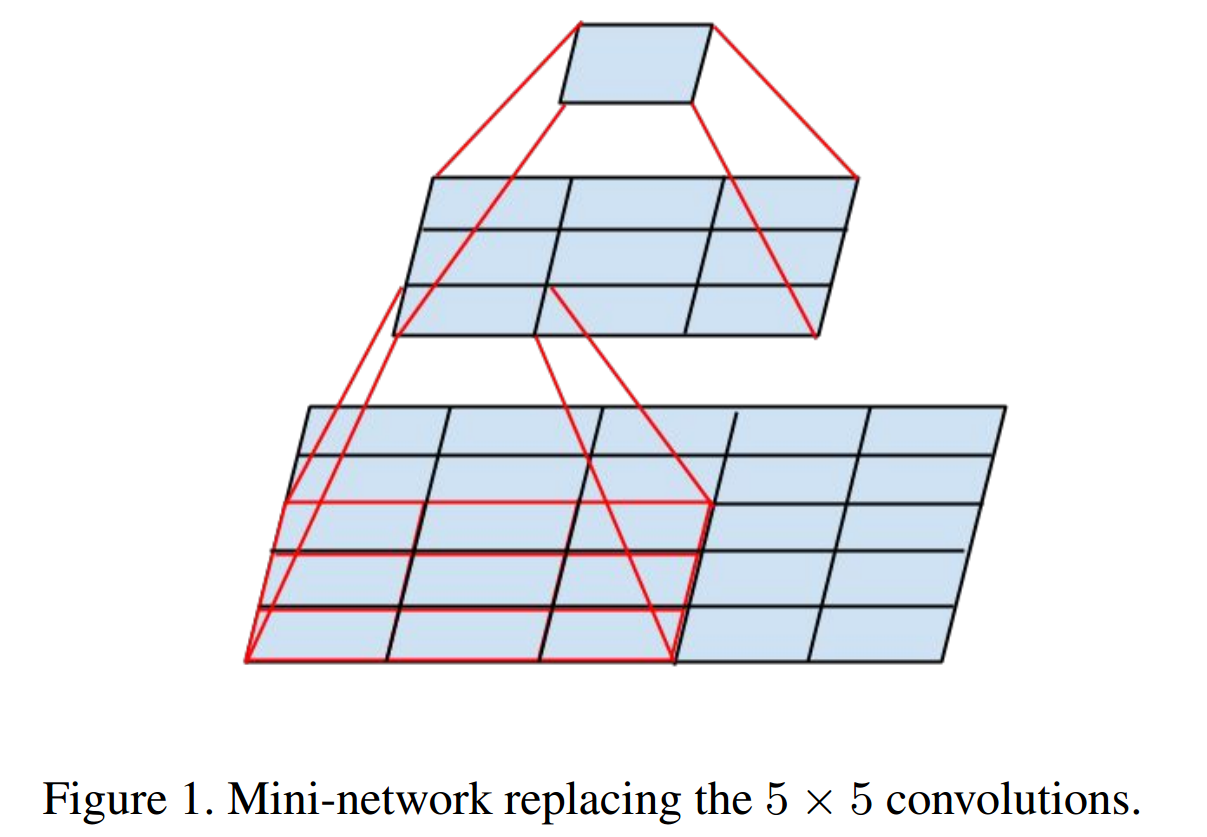
\includegraphics[width=\textwidth]{./figures/edit/5x5.png}
	\end{figure}
\end{frame}

\begin{frame}
  \frametitle{Breakding down Convolution ... (6)}
  Breakding down $3 \times 3$ convolution into $3 \times 1$ and $1 \times 3$ convolutions (assymetric breakdown).
	\begin{itemize}
		\item Let us calculate the average of a $3 \times 3$ matrix.
	\end{itemize}	  
\begin{minipage}{0.15\textwidth}
    \begin{tikzpicture}

    %\matrix[matrix of nodes,nodes={draw},row 										1 2/.style={nodes={fill=blue!20}}] {
    \matrix (m) [matrix of nodes,
        nodes={rectangle,draw, fill=blue!10} ]{
            $9$ && $8$ && $7$ \\
            $6$ && $5$ && $4$ \\
            $3$ && $2$ && $1$ \\
    };
    \end{tikzpicture}
\end{minipage}
\begin{minipage}{0.01\textwidth}
    \ast
\end{minipage} 
\begin{minipage}{0.15\textwidth}
    \begin{tikzpicture}

    %\matrix[matrix of nodes,nodes={draw},row 										1 2/.style={nodes={fill=blue!20}}] {
    \matrix (m) [matrix of nodes,
        nodes={rectangle,draw, fill=blue!10} ]{
            $\frac{1}{9}$ && $\frac{1}{9}$ && $\frac{1}{9}$ \\
            $\frac{1}{9}$ && $\frac{1}{9}$ && $\frac{1}{9}$ \\
            $\frac{1}{9}$ && $\frac{1}{9}$ && $\frac{1}{9}$ \\
    };
    \end{tikzpicture}
\end{minipage}
\begin{minipage}{0.03\textwidth}
    =
\end{minipage} 
\begin{minipage}{0.50\textwidth}
$\frac{9}{9} + \frac{8}{9} + \dots + \frac{2}{9} + \frac{1}{9}$ 
$\equiv$
\textcolor{red}{9(9M + 8A)}
\end{minipage} \\
\begin{minipage}{0.15\textwidth}
    \begin{tikzpicture}

    %\matrix[matrix of nodes,nodes={draw},row 										1 2/.style={nodes={fill=blue!20}}] {
    \matrix (m) [matrix of nodes,
        nodes={rectangle,draw, fill=blue!10} ]{
            $\frac{1}{9}$ && $\frac{1}{9}$ && $\frac{1}{9}$ \\
            $\frac{1}{9}$ && $\frac{1}{9}$ && $\frac{1}{9}$ \\
            $\frac{1}{9}$ && $\frac{1}{9}$ && $\frac{1}{9}$ \\
    };
    \end{tikzpicture}
\end{minipage}
\begin{minipage}{0.01\textwidth}
    =
\end{minipage} 
\begin{minipage}{0.07\textwidth}
    \begin{tikzpicture}

    %\matrix[matrix of nodes,nodes={draw},row 										1 2/.style={nodes={fill=blue!20}}] {
    \matrix (m) [matrix of nodes,
        nodes={rectangle,draw, fill=blue!10} ]{
            $\frac{1}{3}$ \\
            $\frac{1}{3}$ \\
            $\frac{1}{3}$ \\
    };
    \end{tikzpicture}
\end{minipage}
\begin{minipage}{0.15\textwidth}
\begin{tikzpicture}

    %\matrix[matrix of nodes,nodes={draw},row 										1 2/.style={nodes={fill=blue!20}}] {
    \matrix (m) [matrix of nodes,
        nodes={rectangle,draw, fill=blue!10} ]{
            $\frac{1}{3}$ && $\frac{1}{3}$ && $\frac{1}{3}$ \\
    };
\end{tikzpicture} 
\end{minipage} 
\begin{minipage}{0.50\textwidth}
	\vspace{1em}
    $\equiv$
    \textcolor{red}{9(3M + 2A) + 9(3M + 2A)} \\
    \hspace{5em} = \textcolor{red}{9(6M + 4A)} \\
\end{minipage} \\
\begin{itemize}
	\item The average kernel is a \textcolor{red}{separable filter (rank-1 matrix)}. 
\end{itemize}
\end{frame}

\begin{frame}
	\frametitle{Inception Modules ... (1)}
	\begin{figure}
		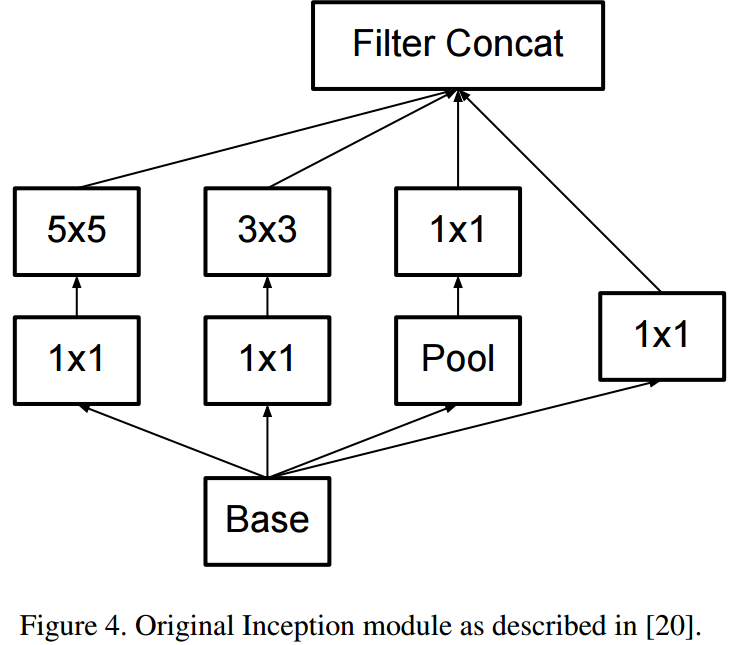
\includegraphics[width=0.45\textwidth]{./figures/edit/inception_org.png}
		\hspace{0.05\textwidth} 
		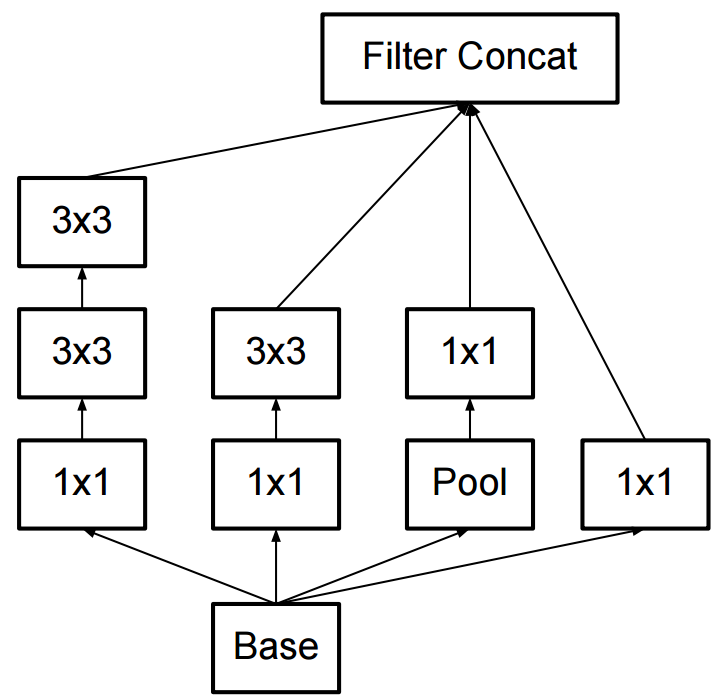
\includegraphics[width=0.45\textwidth]{./figures/edit/breakdown_01.png}
	\end{figure}
\end{frame}

\begin{frame}
	\frametitle{Inception Modules ... (2)}
	\begin{figure}
		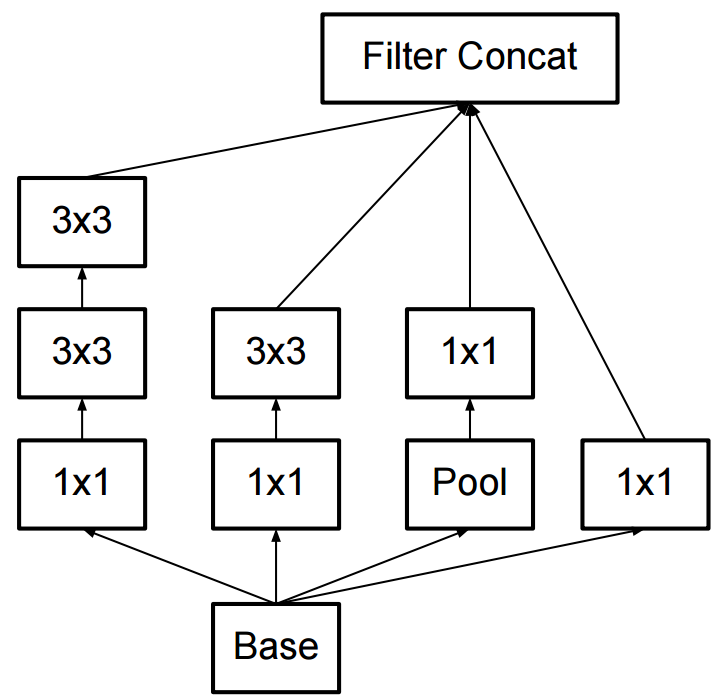
\includegraphics[width=0.45\textwidth]{./figures/edit/breakdown_01.png}
		\hspace{0.05\textwidth} 
		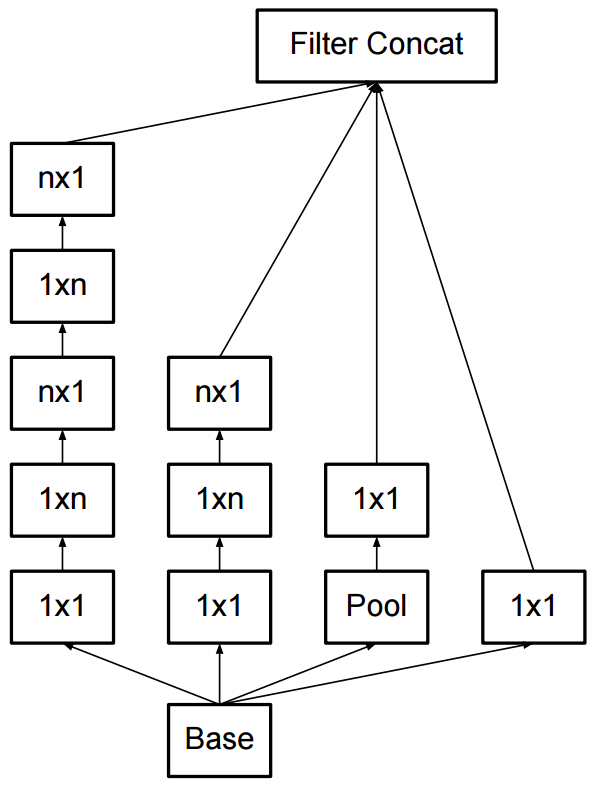
\includegraphics[width=0.45\textwidth]{./figures/edit/breakdown_02.png}
	\end{figure}
\end{frame}

\begin{frame}
	\frametitle{Inception Modules - Final}
	\begin{figure}
		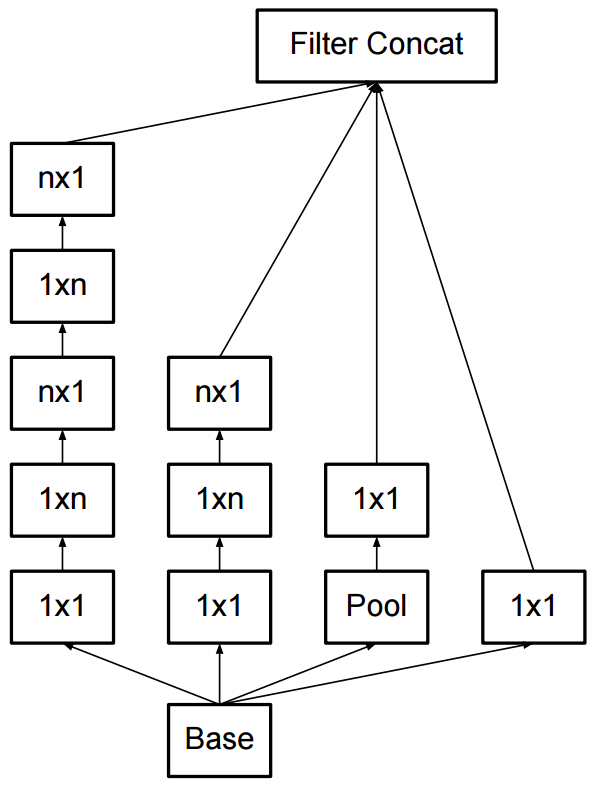
\includegraphics[width=0.45\textwidth]{./figures/edit/breakdown_02.png}
		\hspace{0.05\textwidth} 
		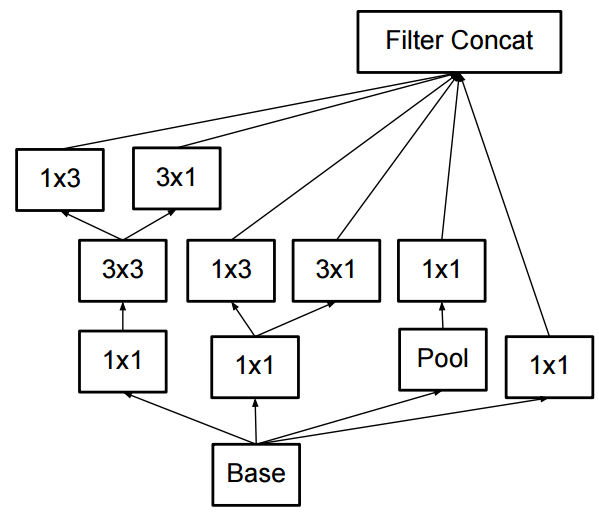
\includegraphics[width=0.45\textwidth]{./figures/edit/breakdown_coarse.png}		
	\end{figure}
\end{frame}

\begin{frame}
	\frametitle{Inception-v3(2014/2016)}
	\begin{figure}
		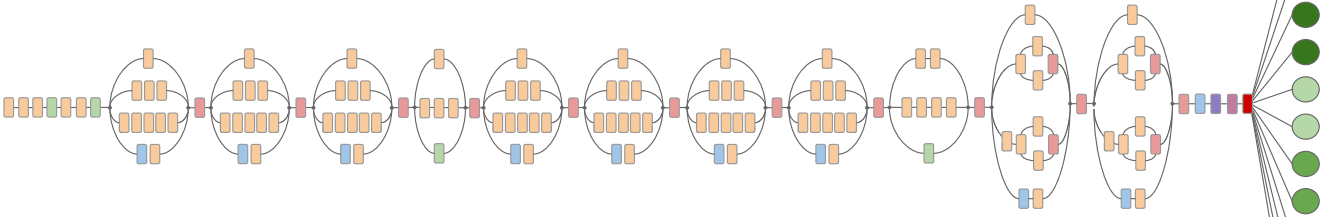
\includegraphics[width=\textwidth, height=4cm]{./figures/edit/inception_v3.png} \\
		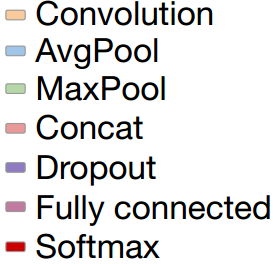
\includegraphics[width=0.2\textwidth]{./figures/edit/inception_layers.png} 
		\hspace{1em}
		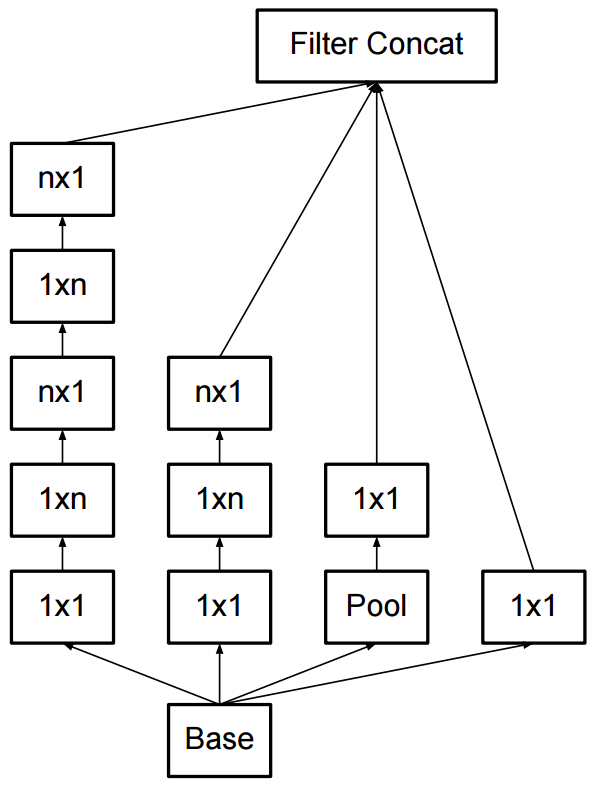
\includegraphics[width=0.35\textwidth, height=3.5cm]{./figures/edit/breakdown_02.png}		
		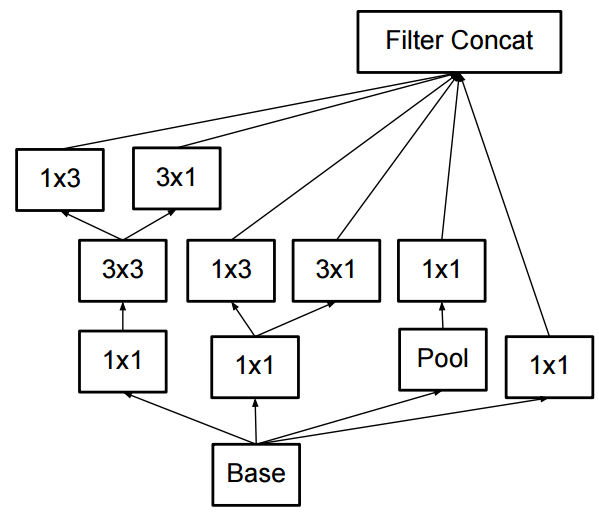
\includegraphics[width=0.35\textwidth, height=3.5cm]{./figures/edit/breakdown_coarse.png}		
	\end{figure}
\end{frame}

\begin{frame}
	\frametitle{Results-Inception}
		\begin{itemize}
			\item Trained for 100 epochs on NVIDIA Kepler GPUs.
		\end{itemize}	
		\begin{table}[]
		\centering
		\label{my-label}
		\begin{tabular}{|c|c|c|}
		\hline
		\multirow{2}{*}{Method} & \multicolumn{2}{c|}{Error (\%)} \\ \cline{2-3} 
		 & Top-1 & Top-5 \\ \hline
		SIFT + FV & 45.7 & 25.7 \\ \hline
		AlexNet & 37.5 & 17.0 \\ \hline
		VGG16 & 24.4 & 7.2 \\ \hline
		VGG19 & 24.4 & 7.1 \\ \hline
		Inception-v3 & 18.8 & 4.2 \\ \hline
		\end{tabular}
		\end{table}
\end{frame}

\subsection{ResNet}

\begin{frame}
	\frametitle{Analysis of Network Depth}
	\begin{itemize}
		\item Simply stacking up lots of convolutional layers make performance worse.	
		\begin{figure}
			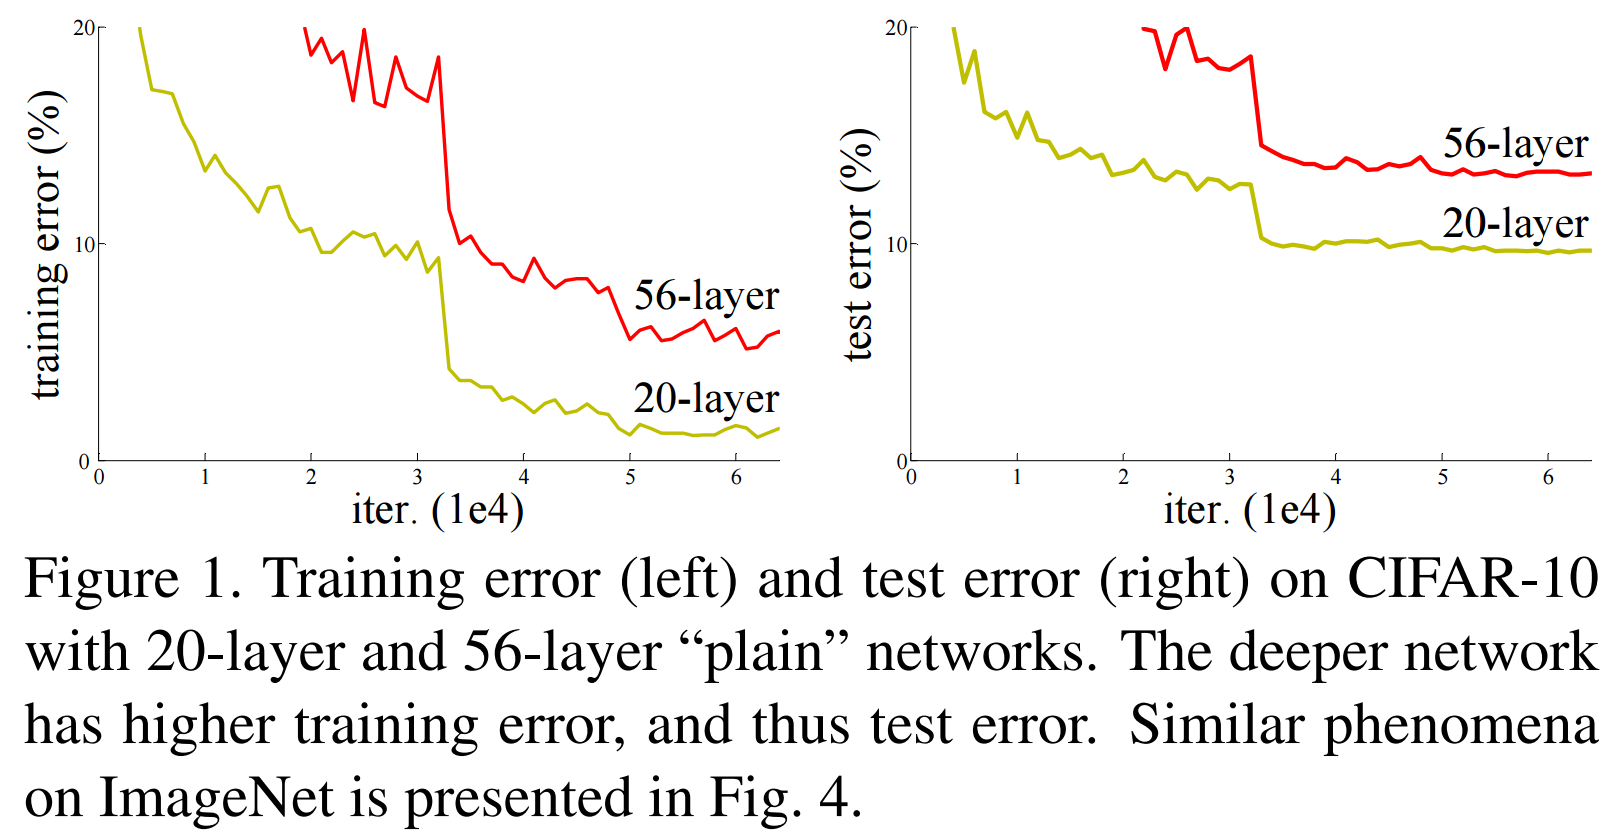
\includegraphics[scale=0.15]{./figures/edit/depth_analysis.png}
		\end{figure}
		\item Current gradient-descent solvers are bad at optimizing the training parameters for identity mapping.
	\end{itemize}
\end{frame}

\begin{frame}
	\frametitle{Learning by Comparison}
	\begin{itemize}
		\item Rather than memorizing from scratch, memorizing the changes with respect to something known makes learning faster.	
		\item Example: You are fluent in English and are now interested to learn French. \\
		\hspace{2em} University (English) -- Universit\'e (French)
		\pause
		\item This idea of ``Learning by Comparison" can be implemented in CNN using shortcut/bypass connections.
	\end{itemize}
	\begin{figure}
		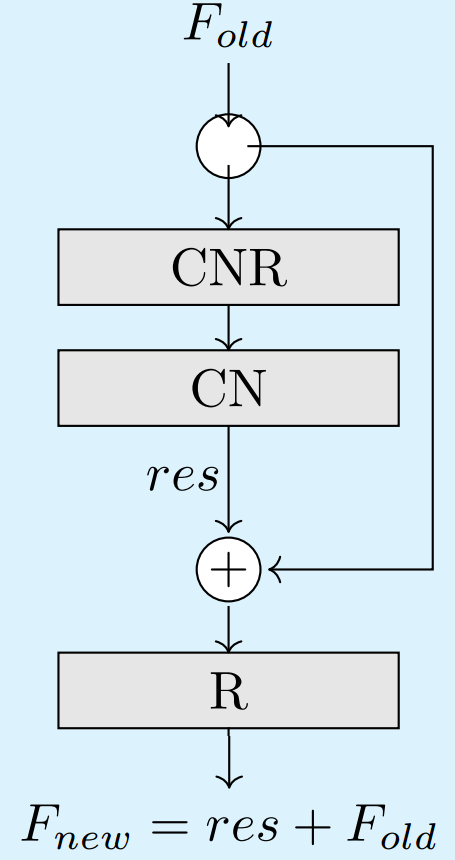
\includegraphics[scale=0.15]{./figures/edit/residual.png}
	\end{figure}
\end{frame}

\begin{frame}
	\frametitle{ResNet(2015)}
	\begin{minipage}[t]{0.25\textwidth}	
		\begin{figure}[t]
			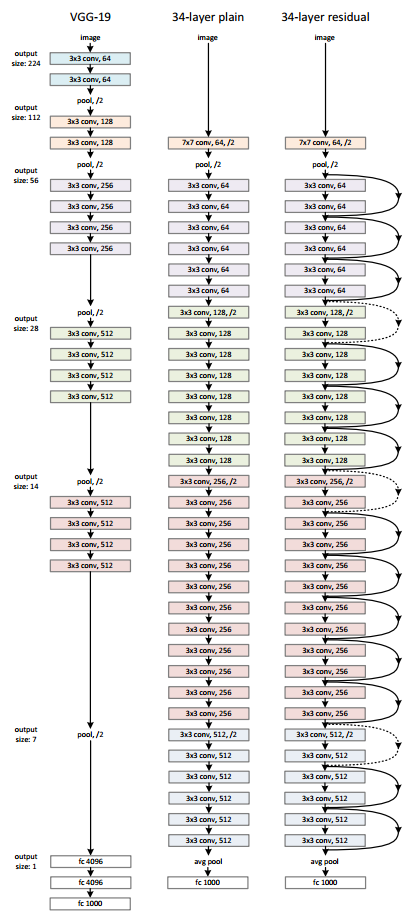
\includegraphics[scale=0.2]{./figures/edit/resnet_arch.png}
		\end{figure}
	\end{minipage}	
	\begin{minipage}[t]{0.70\textwidth}	
		\begin{itemize}
			\item Possible to train of much deeper models than before, e.g. ResNet50, ResNet101, ResNet152.
			\item Deeper models work better.
			\item Use of Global Average Pooling (GAP) instead of Fully Connected (FC) layers.
			\item Use of Batch-Normalization (running estimation of mini-batch mean and std and normalization afterward) instead of Dropout.
		\end{itemize}
		\begin{table}[]
		\centering
		\label{my-label}
		\begin{tabular}{|c|c|c|}
		\hline
		\multirow{2}{*}{Method} & \multicolumn{2}{c|}{Error (\%)} \\ \cline{2-3} 
		 & Top-1 & Top-5 \\ \hline
		SIFT + FV & 45.7 & 25.7 \\ \hline
		AlexNet & 37.5 & 17.0 \\ \hline
		VGG16 & 24.4 & 7.2 \\ \hline
		VGG19 & 24.4 & 7.1 \\ \hline
		Inception-v3 & 18.8 & 4.2 \\ \hline
		ResNet152 & - & 3.57 \\ \hline
		\end{tabular}
		\end{table}
		
	\end{minipage}
\end{frame}

\subsection{DenseNet}
\begin{frame}
	\frametitle{Existing Problems in Deeper Networks}
	\begin{itemize}
		\item Gradienet might still vanish by the time it reaches the end (Vanishing Gradient problem).
		\begin{itemize}
			\item[--] \textcolor{green!70!black} {Possible solution: More Dense connection than shortcut to maximize information flow.} 
		\end{itemize}
		\item Many layers in ResNet contribute very little and can be stochastically dropped.
		\begin{itemize}
			\item[--] \textcolor{green!70!black} {Possible solution: Feature reuse from the previous layers} 
		\end{itemize}		
		\item Computations in ResNet layers are explicit and requires extra memory.
		\begin{itemize}
			\item[--] \textcolor{green!70!black} {Possible solution: Memory reuse.} 
		\end{itemize}
	\end{itemize}
	\pause
	\begin{figure}
		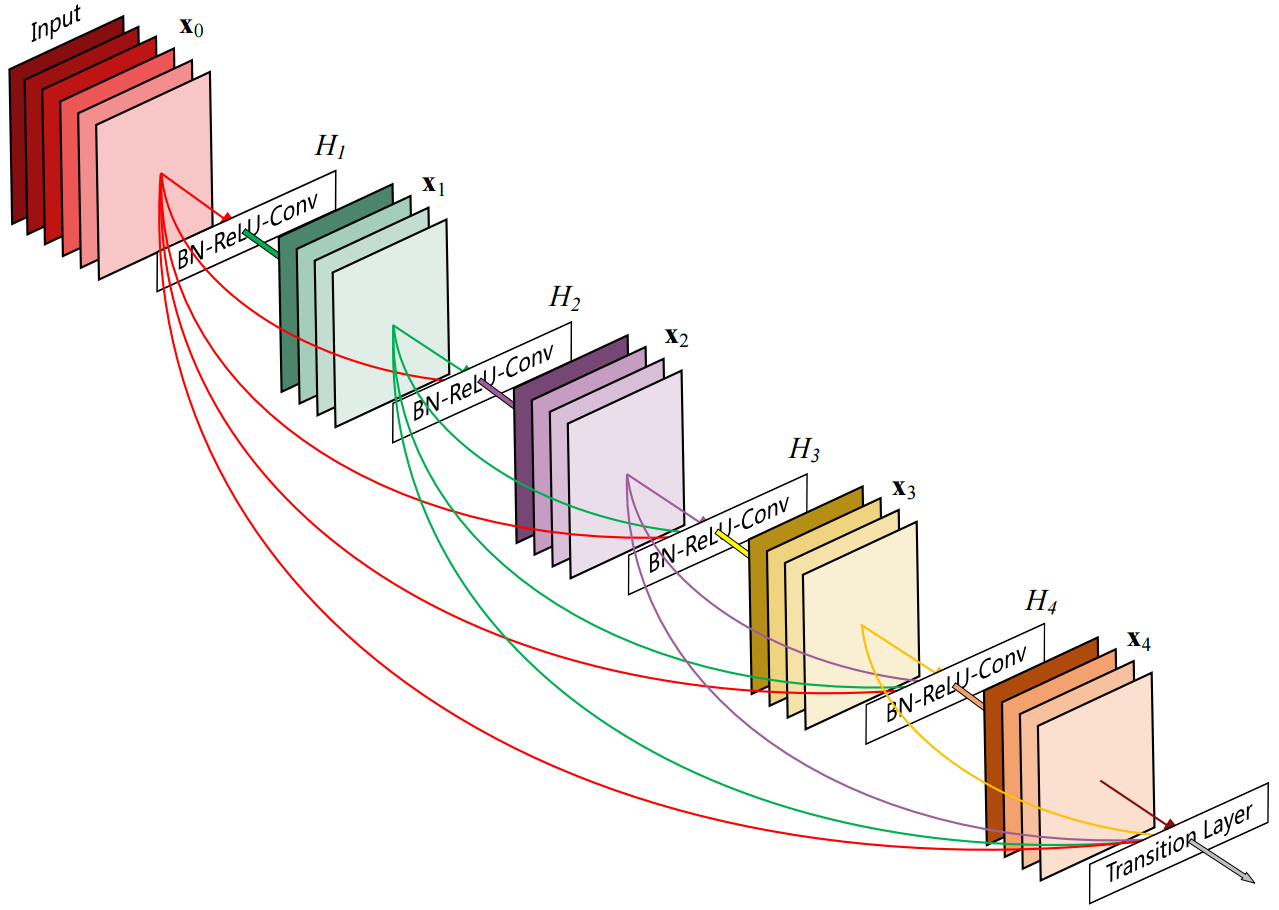
\includegraphics[scale=0.13]{./figures/edit/densenet_01.png}
	\end{figure}
\end{frame}

\begin{frame}
	\frametitle{DenseNet(2017)}
	\begin{figure}
		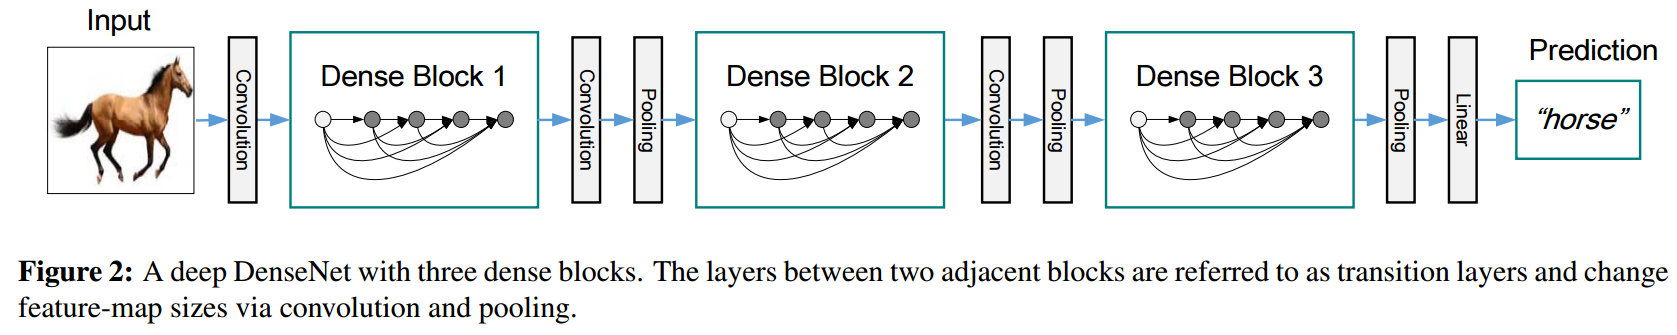
\includegraphics[scale=0.18]{./figures/edit/densenet_02.png} \\
		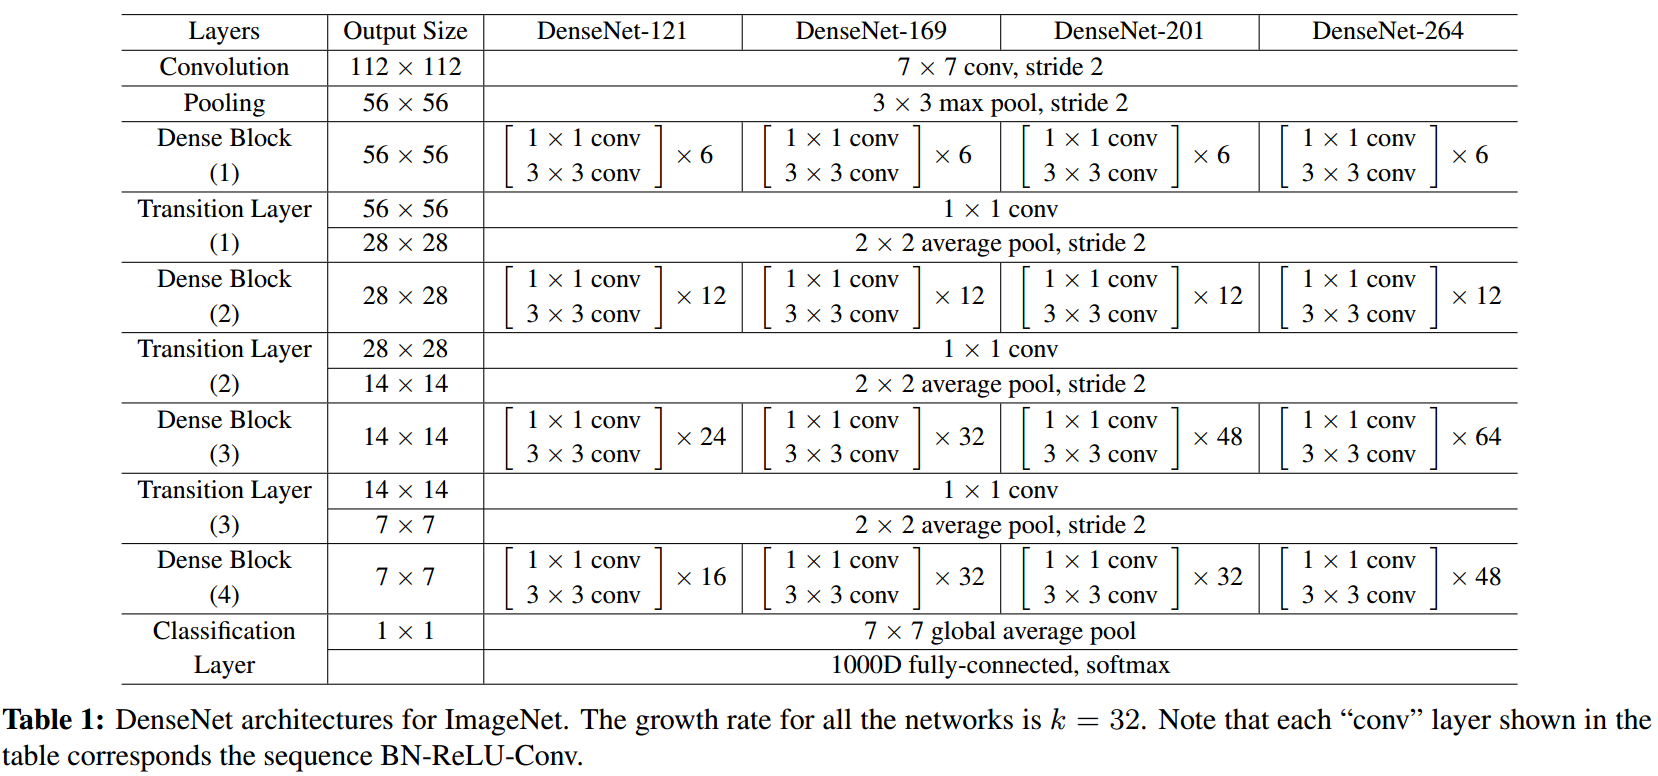
\includegraphics[scale=0.2]{./figures/edit/densenet_03.png} 		
	\end{figure}
\end{frame}

\begin{frame}
	\frametitle{Final Results - Single Crop}
		\begin{table}[]
		\centering
		\caption{Accuracy on Single $224\times 224$ Crop}
		\label{my-label}
		\begin{tabular}{|c|c|c|}
		\hline
		\multirow{2}{*}{Method} & \multicolumn{2}{c|}{Error (\%)} \\ \cline{2-3} 
		 & Top-1 & Top-5 \\ \hline
		AlexNet & 43.45 & 20.91 \\ \hline
		VGG16 + BN & 26.63 & 8.50 \\ \hline
		VGG19 + BN & 25.76 & 8.15 \\ \hline
		Inception-v3 & 22.55 & 6.44 \\ \hline
		ResNet152 & 21.69 & 5.94 \\ \hline
		DenseNet161 & 22.35 & 6.20 \\ \hline
		\end{tabular}
		\end{table}
\end{frame}

\begin{frame}[allowframebreaks]
        \frametitle{References}
        \bibliographystyle{plain}
        \bibliography{image_classification}
\end{frame}

\end{document}


